\section{Propuesta}

\subsection{Descripción}
En esta aplicación vamos a poder realizar diversas acciones en función del rol que tengamos, como explicaremos al inicio de la iteración 0, pero principalmente ésta será una aplicación destinada a la adopción y acogida de animales que lo necesiten. Aquí los usuarios podrán hablar con las asociaciones y enviar solicitudes de adopción y/o acogida, además también podrán anotarse en los voluntariados que ofrezcan las asociaciones y se le facilitará la gestión a las mismas.

También se planea realizar el seguimiento de los animales en adopción desde la propia aplicación con el objetivo de centralizar la gestión de la asociación en un solo sistema.

Por último se contempla la opción de que se pueda apadrinar a los animales desde la propia aplicación.

Adoptapp se implementará tanto para dispositivos móviles como para navegadores web. Se realizarán las pruebas y ajustes necesarios, como se irá viendo a lo largo del desarrollo.

\subsection{Herramientas de desarrollo elegidas}

\subsection{Ciclo de vida/Metodología}
En esta sección hablaremos de la metodología empleada, que en este caso hemos decidido usar la famosa metodología ágil scrum, que vamos a adaptar a nuestro caso.

El desarrollo se va a realizar por una sola persona, el autor de este TFG, el cual mantendrá reuniones periódicas con su tutora, especialmente al inicio y fin de cada iteración o sprint.

Debido a la fluctuación temporal, es posible que haya semanas en las que la carga de trabajo sea elevada, debido a exámenes o trabajos, y no podamos desarrollar la aplicación. Hemos decidido hacer sprints largos de un mes. Con esto tratamos de conseguir obtener un prototipo que va evolucionando con cambios considerables a lo largo de cada sprint.

Vamos a incluir una iteración 0 para describir a los actores del sistema y los requisitos de la aplicación a desarrollar, creando un product backlog de historias de usuario. Calcularemos  su prioridad y haremos una estimación temporal de cada una en puntos de historia.  

\subsection{Iteración 0}
Antes de empezar con la realización de las historias de usuario, debemos tener en cuenta los actores que participarán en la aplicación, los hemos dividido en 5 principales.
\begin{itemize}
	\item \textbf{Usuario básico}: este es el único usuario que no necesitará registrarse en la aplicación, y solo podrá hacer consultas, como por ejemplo ver los animales en adopción o las publicaciones de animales perdido/encontrado.
	\item \textbf{Usuario estándar o particular}: Es el tipo de usuario registrado más común que habrá en la aplicación. Éste podrá, además de lo mencionado para el básico, crear publicaciones de animal perdido/encontrado, acceder a su perfil, hablar con las asociaciones para adoptar o apadrinar un animal y también hacerse voluntarios si hay asociaciones que lo deseen y ayudarlas en lo que necesiten. Otra de sus capacidades será la de reportar publicaciones en caso de que consideren que son indebidas para la aplicación.
	\item \textbf{Asociaciones}: Este tipo de usuarios se caracteriza por ser los únicos que pueden subir publicaciones de animales en adopción. Éstas también podrán gestionar publicaciones de animales perdidos/encontrados y además decidirán si quieren que sus animales puedan ser acogidos o apadrinados. También podrán solicitar voluntarios.
	\item \textbf{Moderadores}: Son los encargados de que las publicaciones subidas a la aplicación sean consistentes, por ejemplo si alguien sube alguna publicación de animal perdido y son fotos de la cara de una persona, los usuarios particulares podrán reportarlo y los moderadores decidirán si eliminarla o no, en este caso la eliminarían. Además se encargarán de validar a las asociaciones que se registren mediante alguna documentación específica.
	\item \textbf{Administradores}: Estos usuarios son los encargados de crear a los moderadores, además podrá crear o eliminar todo tipo de usuarios.
	
\end{itemize}
\subsubsection{Product Backlog}
Para obtener las prioridades hemos hecho uso de MoSCoW \cite{moscow} que es una herramienta de decisión y priorización de tareas y funcionalidades para la gestión de proyectos.

La utilidad principal del método MoSCoW está enfocada en el desarrollo de productos y servicios digitales. Es una herramienta que ayuda a priorizar y gestionar los requisitos y tareas para avanzar.

MoSCoW es un método bastante eficaz en entornos de desarrollo ágil, permitiendo priorizar las funciones necesarias para lanzar un nuevo producto o funcionalidad.

A continuación se mostrará el product backlog, pero vale la pena detenernos a explicar los campos \textit{duración} y \textit{Prio.(prioridad)}.

El primero son los puntos de historia, que pueden tener 1,3,5,8 como valor y se refieren a la estimación de tiempo para la realización de la misma.

La prioridad se marca con las siguientes letras:
\begin{itemize}
	\item  \textbf{M}ust: Estas características serán las absolutamente críticas para el proyecto, y sin ellas es un fracaso.
	\item \textbf{S}hould: Estos aspectos del proyecto son críticos también, pero no imprescindibles.
	\item \textbf{C}ould: Estas iniciativas son las que estaría bien tenerlas, ya que añadirían valor al proyecto, pero no son críticas.
	\item \textbf{W}on't: Estas características no se merecen la inversión y no aportan ningún beneficio en este momento y se podrían considerar más tarde.
\end{itemize}

Antes de la creación de las historias de usuario hemos mantenido una entrevista con la asociación de \href{https://www.instagram.com/coloniasfelinasarmilla/}{Colonias felinas Armilla} la cual nos ha permitido concretar mejor los requisitos de la aplicación.

\begin{table}[H]
	\centering
	\begin{tabular}{|c |p{8cm}|c |c|} \hline 
		\multirow[c]{3}{*}{Usuario}&  \textbf{Tarea}&  \textbf{Duración}& \textbf{Prio.}\\  \cline{2-4}%Prio. es de prioridad 
		&  Acceder a la aplicación&  5& M\\ \cline{2-4} 
		&  Cerrar sesión&  1& M\\ \hline 
	\end{tabular}
	\caption{Product backlog de usuarios}
	\label{tab:pb_usuarios}
\end{table}

\begin{table}[H]
	\centering
	\begin{tabular}{|c |p{8cm}|c |c|} \hline 
		\multirow[c]{25}{*}{Asociación}&  \textbf{Tarea}&  \textbf{Duración}& \textbf{Prio.}\\  \cline{2-4}
		
		&  Registrarme en la aplicación como asociación&  5& M\\ \cline{2-4} 
		&  Crear publicación de animal en adopción&  8& M\\ \cline{2-4} 
		&  Anular poner animal en adopción&  3& M\\ \cline{2-4} 
		&  Ver solicitudes de adopción por parte de los particulares&  5& M\\ \cline{2-4}
		&  Aceptar solicitudes de adopción&  3& M\\ \cline{2-4}
		&  Rechazar solicitudes de adopción&  3& M\\ \cline{2-4}
		
		
		&  Poner animales en acogida&  3& M\\ \cline{2-4}
		&  Anular poner animal en acogida&  3& M\\ \cline{2-4} 
		&  Ver solicitudes de acogida por parte de los particulares&  3& M\\ \cline{2-4}
		
		&  Ver qué particulares tienen a sus animales en acogida&  5& M\\ \cline{2-4}
		&  Buscar particulares que estén como casa de acogida&  5& M\\ \cline{2-4}
		&  Solicitar acogida a particular puesto como casa de acogida &  5& M\\ \cline{2-4}
		
		
		&  Decidir si desean ser voluntarios o no&  3& M\\ \cline{2-4}
		&  Ver solicitudes voluntariado propias&  3& M\\ \cline{2-4}
		&  Aceptar solicitudes voluntariado&  3& M\\ \cline{2-4}
		&  Rechazar solicitudes voluntariado&  3& M\\ \cline{2-4}
		
		&  Mandar contrato adopción firmado al adoptante&  8& S\\ \cline{2-4}
		
		&  Elegir si poner a sus animales como apadrinables o no &  5& S\\ \cline{2-4}
		
		&  Modificar su descripción para que los usuarios vean a qué se dedican & 5 & M \\ \hline
		
		
		
		
	\end{tabular}
	\caption{Product backlog de Asociaciones}
	\label{tab:pb_asociaciones}
\end{table}


\begin{table}[H]
	\centering
	\begin{tabular}{|c |p{8cm}|c |c|} \hline 
		\multirow[c]{14}{*}{Particular}&  \textbf{Tarea}&  \textbf{Duración}& \textbf{Prio.}\\  \cline{2-4}
		&  Registrarme en la aplicación como particular&  5& M\\ \cline{2-4} 
		
		
		&  Solicitar adopciones&  3& M\\ \cline{2-4}
		&  Ver adopciones pendientes&  3& S\\ \cline{2-4}
		
		&  Solicitar acogidas&  3& M\\ \cline{2-4} 
		&  Ver acogidas pendientes&  3& M\\ \cline{2-4}
		
		&  Ponerse como casa de acogida&  3& S\\ \cline{2-4}
		
		&  Cumplimentar el formulario de solicitud de adopciones/acogidas &  5& S\\ \cline{2-4}
		&  Firmar contrato de adopción electrónicamente&  8& S\\ \cline{2-4}
		
		
		&  Solicitar realización de voluntariado&  3& M\\ \cline{2-4} 
		&  Ver servicios de voluntariado pendientes&  3& M\\ \cline{2-4}
		&  Ver historial de servicios de voluntariado&  5& C\\ \cline{2-4}
		
		
		& Apadrinar a un animal&  5& S\\ \hline
		
		
		
	\end{tabular}
	\caption{Product backlog de Particulares}
	\label{tab:pb_particulares}
\end{table}

\begin{table}[H]
	\centering
	\begin{tabular}{|c |p{8cm}|c |c|} \hline 
		\multirow[c]{16}{2cm}{Asociación y Particular}&  \textbf{Tarea}&  \textbf{Duración}& \textbf{Prio.}\\  \cline{2-4}
		
		&  Ver su perfil &  5& M\\ \cline{2-4}
		&  Modificar su perfil &  5& M\\ \cline{2-4}
		&  Eliminar su perfil &  3& M\\ \cline{2-4}
		
		&  Aceptar solicitudes acogida&  3& M\\ \cline{2-4}
		&  Rechazar solicitudes acogida&  3& M\\ \cline{2-4}
		
		&  Ver historial de adopciones &  5& M\\ \cline{2-4}
		&  Ver historial de acogidas &  5& M\\ \cline{2-4}
		&  Eliminar publicación de animal perdido/encontrado &  3& M\\ \cline{2-4}
		
		& Añadir publicación de animal perdido o encontrado & 5 & M \\ \cline{2-4}
		
		
		&  Reportar un perfil &  1& M\\ \cline{2-4}
		&  Reportar una publicación &  1& M\\ \cline{2-4}
		
		&  Realizar el seguimiento de adopción por parte de la asociación al adoptante&  8& C\\ \cline{2-4}
		
		&  Chatear con otros usuarios a raíz de una adopción/acogida/voluntariado &  8& M\\ \hline
		
		
		
	\end{tabular}
	\caption{Product backlog de Particulares y Asociaciones}
	\label{tab:pb_aso_particular}
\end{table}

\begin{table}[H]
	\centering
	\begin{tabular}{|c |p{8cm}|c |c|} \hline 
		\multirow[c]{4}{2cm}{Us. Básico y Particular}&  \textbf{Tarea}&  \textbf{Duración}& \textbf{Prio.}\\  \cline{2-4}
		& Ver lista de animales perdidos/encontrados & 5 & M \\ \cline{2-4}
		&  Buscar publicaciones en una zona concreta&  5& S\\ \cline{2-4}		
		&  Ver peticiones de adopción&  8& M\\ \hline
		
		
		
	\end{tabular}
	\caption{Product backlog de Us. Básico y Particulares}
	\label{tab:pb_part_usBasico}
\end{table}

\begin{table}[H]
	\centering
	\begin{tabular}{|c|p{8cm}|c|c|} \hline 
		\multirow[c]{4}{*}{Administrador}&  \textbf{Tarea}&  \textbf{Duración}& \textbf{Prio.}\\  \cline{2-4}
		&  Crear usuarios &  5& M\\ \cline{2-4}
		&  Modificar usuarios &  5& M\\ \cline{2-4}
		&  Eliminar usuarios &  3& M\\ \hline
		
		
		
	\end{tabular}
	\caption{Product backlog de Administradores}
	\label{tab:pb_administradores}
\end{table}

\begin{table}[H]
	\centering
	\begin{tabular}{|c|p{8cm}|c|c|} \hline 
		\multirow[c]{7}{*}{Moderador}&  \textbf{Tarea}&  \textbf{Duración}& \textbf{Prio.}\\  \cline{2-4}
		&  Ver publicaciones reportadas &  5& M\\ \cline{2-4}
		&  Eliminar publicaciones &  3& M\\ \cline{2-4}
		
		&  Ver usuarios reportados &  5& M\\ \cline{2-4}
		&  Impedir acceso a usuarios reportados &  3& M\\ \cline{2-4}
		
		&  Ver lista de asociaciones recién registradas &  5& M\\ \cline{2-4}
		&  Validar las asociaciones recién registradas& 5 & M\\ \hline
		
		
		
	\end{tabular}
	\caption{Product backlog de Moderadores}
	\label{tab:pb_moderadores}
\end{table}

Una vez creadas todas las historias de usuario y considerando el tiempo estimado para realizar cada una, procedemos a su planificación y asignación en los diferentes sprints. Como hemos comentado, la idea es seguir la metodología Scrum con sprints de un mes.  \\

La  velocidad del sprint será aproximadamente de unos 35-40 puntos. Esta estimación es muy subjetiva y puede variar con el tiempo ya que no se tienen sprints anteriores con los que calcular dicha velocidad de manera más meticulosa.

Hablando con las asociaciones nos hemos dado cuenta de que los intercambios de acogidas no son una buena idea, ya que según la protectora sería fácil perder el control del animal en cuestión, por lo que se han descartado las historias de usuario relacionadas con las acogidas. \\

A continuación se muestran las tareas asignadas a cada sprint, para la administración del trabajo hemos utilizado la herramienta \textit{JIRA} y lo que se muestra son capturas de la misma: \\

Sprint 1 \\ 
\begin{figure}[H]
	\centering
	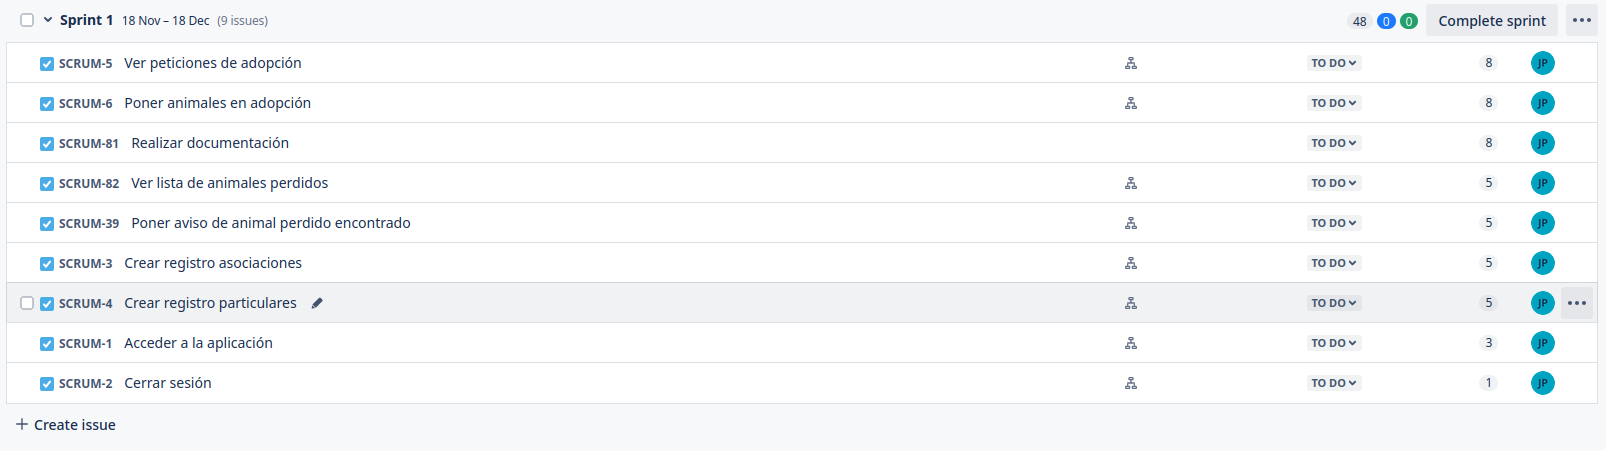
\includegraphics[width=1\linewidth]{screenshot001}
	\caption{Planificación del primer sprint}
	\label{fig:sprint1}
\end{figure}


Sprint 2 \\
\begin{figure}[H]
	\centering
	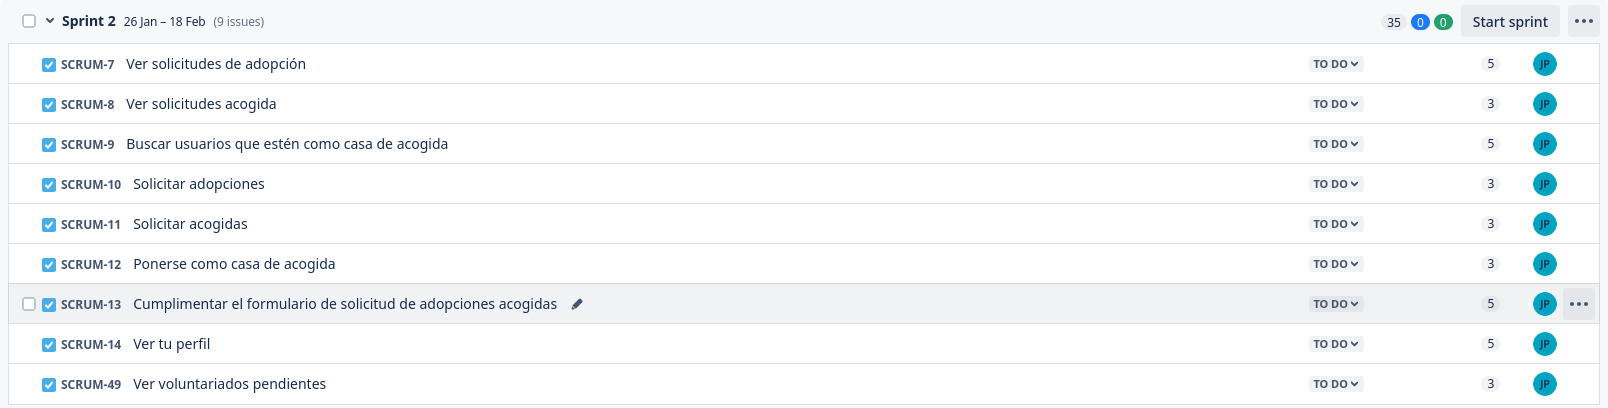
\includegraphics[width=1\linewidth]{screenshot002}
	\caption{Planificación del segundo sprint}
	\label{fig:sprint2}
\end{figure} 


Sprint 3 \\ 
\begin{figure}[H]
	\centering
	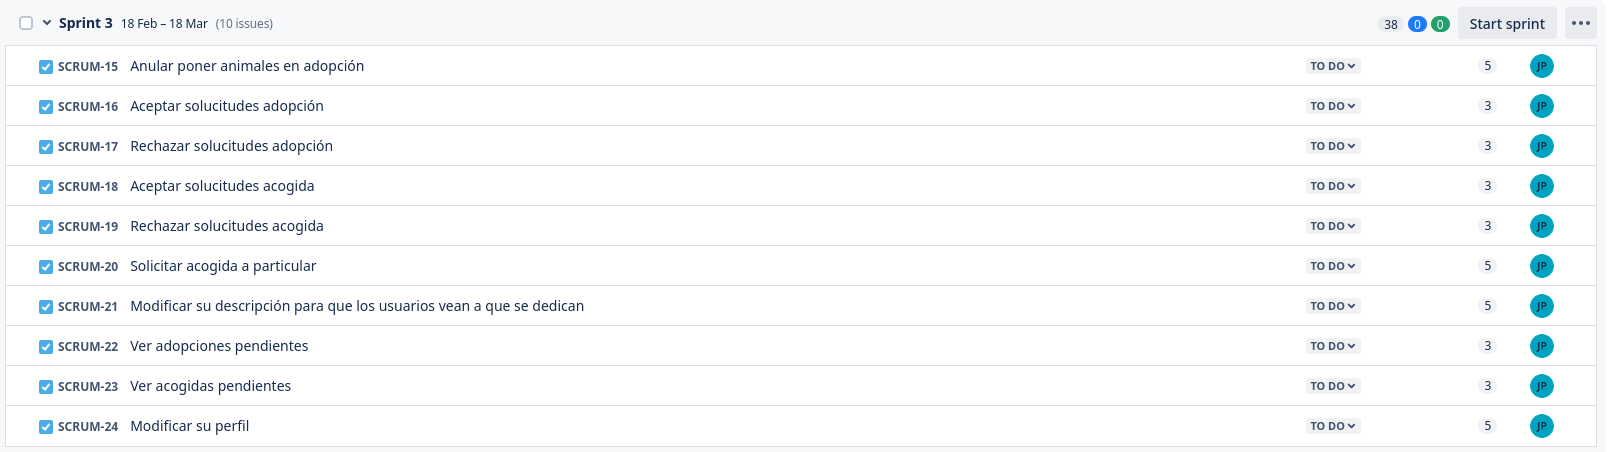
\includegraphics[width=1\linewidth]{sprint3}
	\caption{Planificación del tercer sprint}
	\label{fig:sprint3}
\end{figure}

Sprint 4 \\
\begin{figure}[H]
	\centering
	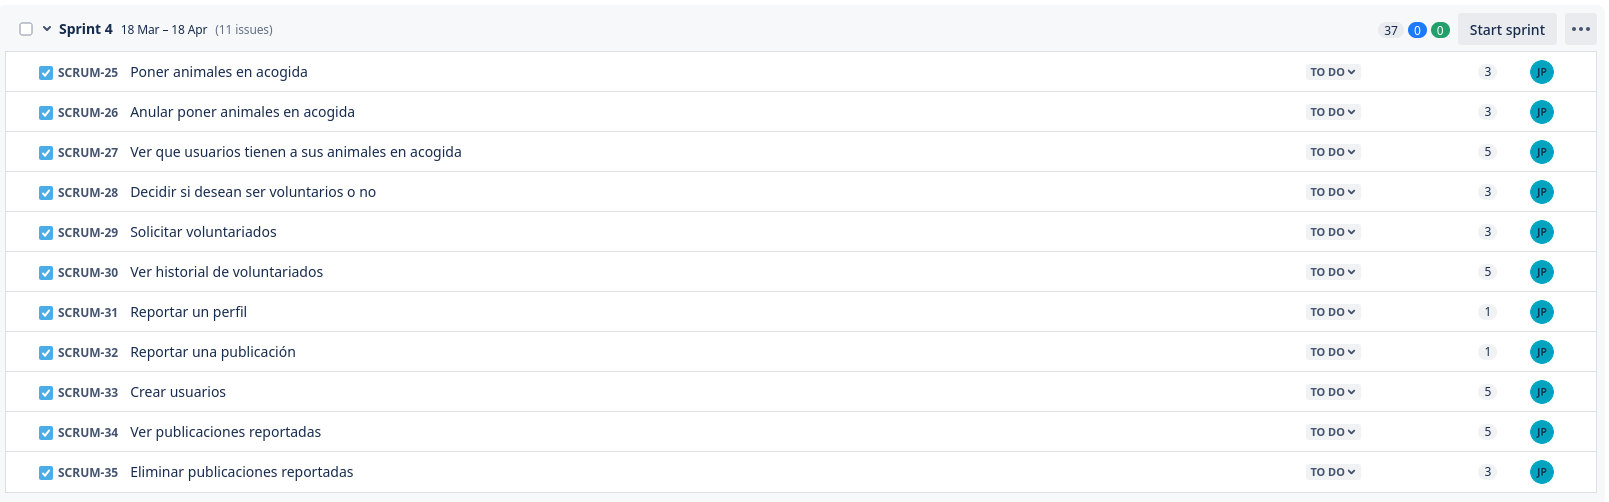
\includegraphics[width=1\linewidth]{sprint4}
	\caption{Planificación del cuarto sprint}
	\label{fig:sprint4}
\end{figure}

Sprint 5 \\ 
\begin{figure}[H]
	\centering
	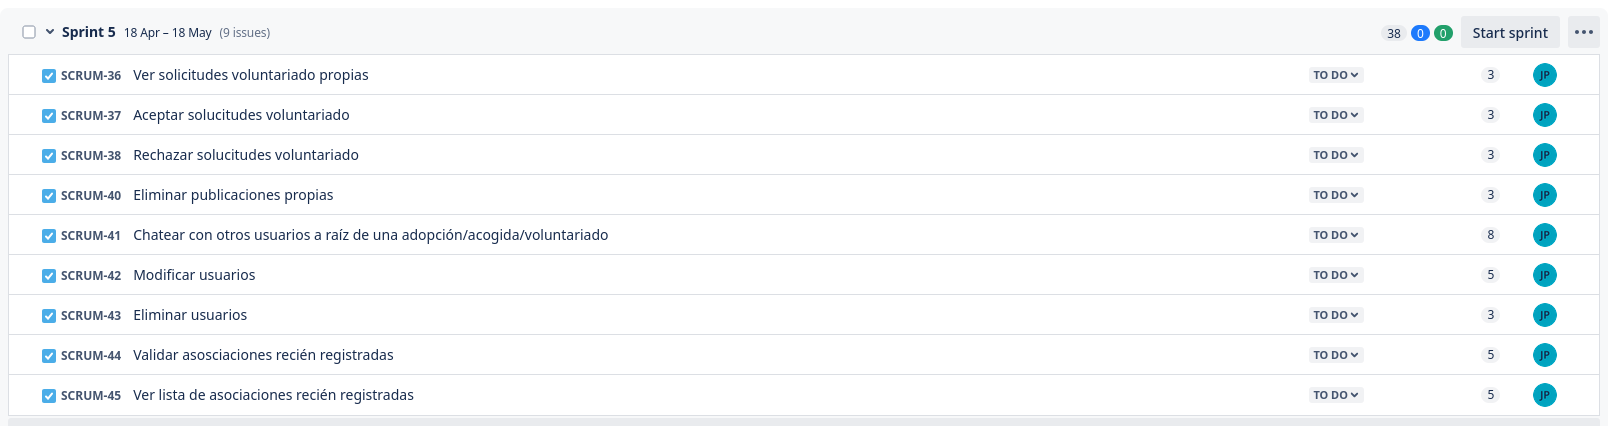
\includegraphics[width=1\linewidth]{sprint5}
	\caption{Planificación del quinto sprint}
	\label{fig:sprint5}
\end{figure}

Product backlog restante \\
\begin{figure}[H]
	\centering
	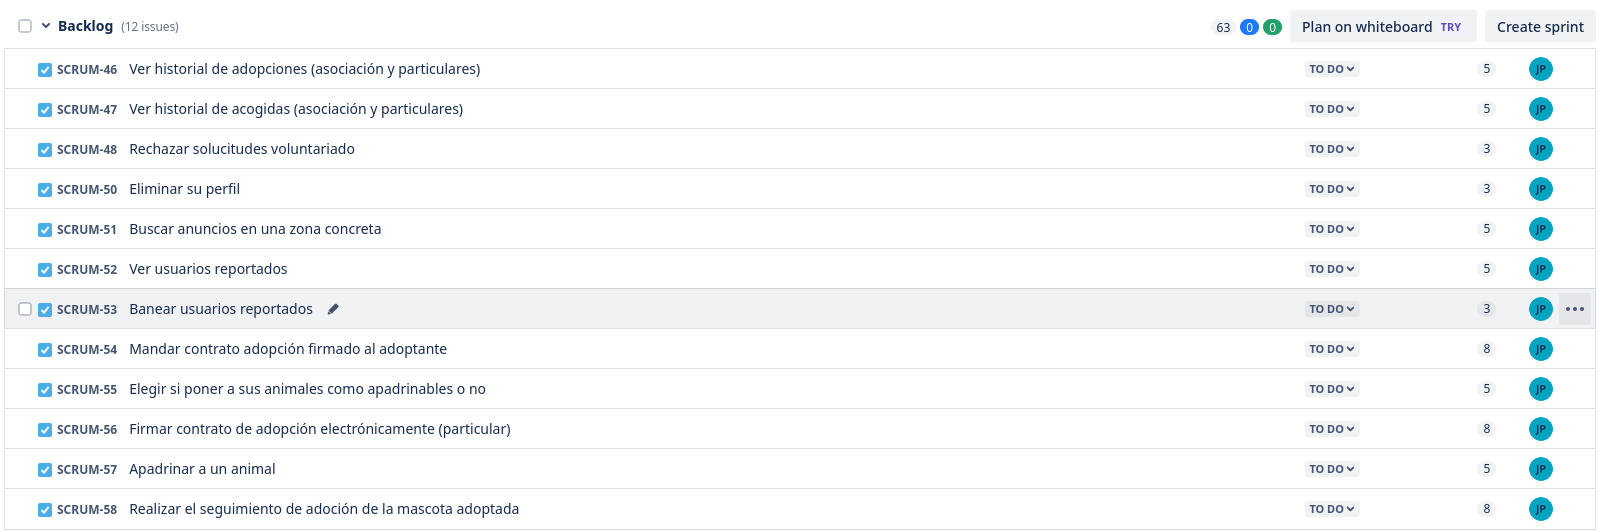
\includegraphics[width=1\linewidth]{pb}
	\caption{Tareas a hacer en siguientes sprints}
	\label{fig:pb_restante}
\end{figure}





\subsection{Iteración 1}

\large{En esta iteración se realizarán las historias que hacen referencia a los animales en adopción y su documentación asociada. Hay pocas historias de usuario debido a que en esta iteración también se realizará el aprendizaje de las tecnologías a utilizar y la preparación de la arquitectura, por lo que el desarrollo será más lento.}
 \\ 

\large{\textbf{Especificación de tareas}} \\


\begin{tabular}{|c|p{9.5cm}|p{1cm}|}
	\hline
	\multicolumn{3}{|c|}{\textbf{HU.1 - Ver animales en adopción}} \\
	\hline
	\textbf{Id} & \textbf{Título de la tarea de desarrollo} & \textbf{Est. (días)} \\
	\hline
	1.1 & Realizar bocetos & 0.5 \\ \hline
	1.2 &  Implementar interfaz para ver las adopciones disponibles & 2 \\ \hline
	1.3 &  Implementar la lógica de obtención de animales en adopción & 1 \\ \hline
	1.4 &  Diseño y creación de la base de datos y tablas & 1 \\ \hline
	\multicolumn{3}{|c|}{\textbf{Pruebas de aceptación}} \\ \hline
	1 & \multicolumn{2}{|l|}{Mostrar mensaje en caso de que no haya animales} \\ \hline
	2 & \multicolumn{2}{|l|}{Mostrar lista de todos los animales con diferentes filtros de consulta} \\ \hline
	3 & \multicolumn{2}{|l|}{Que los filtros funcionen correctamente} \\ \hline
	
\end{tabular} \\ \\

\label{sec:hu1}

\begin{tabular}{|c|p{9.5cm}|p{1cm}|}
	\hline
	\multicolumn{3}{|c|}{\textbf{HU.2 - Crear publicación de animal en adopción}} \\
	\hline
	\textbf{Id} & \textbf{Título de la tarea de desarrollo} & \textbf{Est. (días)} \\ %Est. es estimación
	\hline
	2.1 & Realizar bocetos & 0.5 \\ \hline
	2.2 &  Implementar formulario con selección y previsualización de imágenes antes de subirlas al servidor para añadir un animal en adopción & 2 \\ \hline
	2.3 &  Insertar datos de animales en la bd & 2 \\ \hline
	2.4 & Modificar la base de datos & 0,5 \\ \hline
	2.5 & Validar los campos introducidos & 0,5 \\ \hline
	\multicolumn{3}{|c|}{\textbf{Pruebas de aceptación}} \\ \hline
	1 & \multicolumn{2}{|l|}{Mostrar avisos en caso de error en el formulario} \\ \hline
	2 & \multicolumn{2}{|l|}{Previsualizar imágenes asociadas al animal} \\ \hline
	3 & \multicolumn{2}{|l|}{Poder eliminar imágenes concretas antes subirlas al servidor} \\\hline
	4 & \multicolumn{2}{|l|}{Comprobar que el animal se ha añadido correctamente a la base de datos} \\\hline
	
\end{tabular} \\ \\


\begin{tabular}{|c|p{9.5cm}|p{1cm}|}
	\hline
	\multicolumn{3}{|c|}{\textbf{HUT.1 - Aprender las tecnologías a utilizar}} \\
	\hline
	\textbf{Id} & \textbf{Título de la tarea de desarrollo} & \textbf{Est. (días)} \\
	\hline
	2.1 & Buscar documentación sobre sequelize & 1,5 \\ \hline
	2.2 & Buscar documentación sobre Ionic & 1,5 \\ \hline
\end{tabular} \\ \\

\begin{tabular}{|c|p{9.5cm}|p{1cm}|}
	\hline
	\multicolumn{3}{|c|}{\textbf{HUT.2 - Instalar y preparar el entorno de desarrollo}} \\
	\hline
	\textbf{Id} & \textbf{Título de la tarea de desarrollo} & \textbf{Est. (días)} \\
	\hline
	2.1 & Instalar programas necesarias & 0,5 \\ \hline
	2.2 & Preparar entorno instalando las librerías pertinentes & 1,5 \\ \hline
\end{tabular} \\ \\


Una vez planificadas todas las historias de usuario del sprint empezaremos a realizarlas preferentemente en el orden designado. \\ \\

\Large{\textbf{HU.1 - Ver animales en adopción}} \\

En esta historia nos encargamos de la visualización de los distintos animales de adopción y su filtrado en función a unos parámetros clave, en este caso se han elegido la edad, la especie, y la localización. \\

Además, por otra parte, cabe destacar que ésta será la página inicial para los usuarios particulares. \\ 

\textbf{Bocetos}

Lo primero es crear los bocetos de la página; para ello, hemos hecho uso de la herramienta draw.io, la cual permite realizar bocetos simples en poco tiempo. Esta herramienta se usará para todos los bocetos.

\begin{figure}[H]
	\centering
	\includegraphics[width=0.31\linewidth]{"bocetos/iteracion 1/adopciones"}
	\caption{Boceto de visualización de animales en adopción}
	\label{fig:adopciones}
\end{figure}

Como podemos ver, la idea para la página es mostrar una lista con los animales en búsqueda de adopción en un contenedor con el siguiente formato:

\begin{itemize}
	\item \textbf{Imágenes de los animales}: Esto será un carrusel de imágenes en el que las asociaciones podrán mostrar el aspecto físico de sus animales.
	\item \textbf{Información específica}: Aquí se encontrarán datos como el nombre, la raza y la edad del animal, además de una descripción sobre el mismo.
	\item \textbf{Botones de acción}: las diferentes acciones a realizar serían la de solicitud de adopción, solicitud de acogida y apadrinamiento. Solicitud y apadrinamiento aparecerán solo si quiere la asociación y el apadrinamiento tampoco aparecerá si ya está apadrinado.
\end{itemize}

\textbf{Implementación} %dimensiones móvil 506x901 \\

\begin{figure}[H]
	\centering
	\includegraphics[width=0.5\linewidth]{"Diseños finales/Iteracion 1/adopciones"}
	\caption{Vista final de la página que muestra a los animales en adopción en móviles}
	\label{fig:adopcionesDef}
\end{figure}


\begin{figure}[H]
	\centering
	\includegraphics[width=0.8\linewidth]{"Diseños finales/Iteracion 1/adopciones_web"}
	\caption{Vista final de la página que muestra a los animales en adopción en web}
	\label{fig:adopcionesDefWeb}
\end{figure}
Para la implantación de todas las historias de usuario usaremos las herramientas elegidas anteriormente, usaremos ionic basado en Angular para la aplicación del cliente y node.js con sequelize como ORM en el servidor. Para esto debemos instalar los paquetes necesarios que en este caso se descargan todos con el comando \textit{npm install "nombre del paquete"}.

En la parte de ionic debemos crear una página con el comando \textit{ionic generate page "nombre de la página"}, a parir de ahí obtenemos 3 archivos principales uno html donde organizaremos la información con etiquetas tanto html como propias de ionic, otro archivo de typescript en el que se encontrará la lógica del cliente y el último es un archivo scss, que es una ampliación del css en el que por ejemplo se pueden anidar clases de estilos y usar variables, en el que estableceremos el diseño de la página.

Como podemos apreciar en ambos diseños se mantienen los componentes principales que mencionamos en los bocetos. Se ha usado la etiqueta \textit{ion-card} de ionic para cada animal y en él se han añadido las imágenes pertinentes obtenidas del servidor, el cual ha hecho una consulta a la base de datos, y una descripción del mismo.

A diferencia de la versión móvil, en web para que el espacio no esté totalmente vacío se ha decidido poner 2 tarjetas por fila, manteniendo su legibilidad y organización básica. \\

Debemos saber que la implementación abarca 3 partes, la implementación del cliente(aplicación ionic) servidor(node.js) y base de datos(mySql).

Para esta HU hemos tenido que crear las tablas en la base de datos de animales, usuarios de tipo asociación, países y provincias, esta última para poder hacer funcionar el filtro de localización para la búsqueda de adopciones. Al final de esta iteración se mostrará un diagrama con la estructura de la base de datos.\\

En cuanto al servidor, se han tenido que crear funciones para obtener a todos los animales o buscarlos en función de los filtros utilizados. \\

En la parte del cliente básicamente se ha creado la pantalla de vista de animales y un servicio de ionic (generado con el comando \textit{ionic generate service nombre-servicio} el cual nos permite conectarnos al servidor mediante una petición http para hacer las peticiones de obtención tanto de los filtros para las búsquedas como de las adopciones que concuerden con los filtros especificados. \\ 



\Large{\textbf{HU.2 - Crear publicación de animal en adopción}}


En esta historia nos encargamos de la subida de animales en adopción a la plataforma para que luego los distintos usuarios los puedan visualizar. \\

\textbf{Bocetos}

\begin{figure}[H]
	\centering
	\includegraphics[width=0.31\linewidth]{"bocetos/iteracion 1/poner-adopción"}
	\caption{Boceto de página para añadir animales en adopción}
	\label{fig:poner-adopcion}
\end{figure}

Podemos apreciar que en esta página será básicamente un formulario que se divide en 3 partes diferenciadas: \\ 

\begin{itemize}
	\item \textbf{Datos básicos}: Este apartado contendrá la información necesaria (nombre, edad, especie, etc.) del animal en cuestión.
	\item \textbf{Imágenes}: En este apartado se pondrán las fotos que se quiera.
	\item \textbf{Datos específicos}: Estos son un conjunto de \textit{checkboxes} en los que se dará información  clínica sobre tratamientos a los que haya sido sometido el animal, como por ejemplo castración o desparasitación entre otros, esto se me ha ocurrido gracias a la aplicación de \textit{Amazdog}, ya que tienen algo similar.
\end{itemize}

\textbf{Implementación} \\

\begin{figure}[H]
	\centering
	\includegraphics[width=0.7\linewidth]{"Diseños finales/Iteracion 1/subidaAdopciones"}
	\caption{ Diseño de subida de adopciones móvil}
	\label{fig:subidaadopciones}
\end{figure}


\begin{figure}[H]
	\centering
	\includegraphics[width=1\linewidth]{"Diseños finales/Iteracion 1/subAdopWeb2"}
	\caption{Diseño de subida de adopciones web}
	\label{fig:subadopweb}
\end{figure}

Como podemos apreciar en diferencia con el boceto, los campos básicos aparecen en vertical de uno en uno en lugar de ir por bloques, esto se ha decido para aportar mayor legibilidad y orden, ya que de la otra manera tendrían tamaños irregulares y en ciertos modelos de teléfono probablemente hubiese errores de superposición de elementos. \\

Para esta historia de usuario se ha modificado la tabla de animales creada para la historia previa para añadir los campos del checkbox y su correspondiente actualización en el backend. También hemos creado métodos para la subida de imágenes, que se guardan en la carpeta uploads del servidor y se enlaza con una tupla en la tabla \textit{images} en la base de datos, la cual contiene su nombre, y el id del animal al que pertenece. En caso de que no se puedan añadir las imágenes por algún error de conexión con el servidor, se borrará de la base de datos al animal y se le avisará al usuario de que ha habido un error. \\


En cuanto al frontend hemos creado una página nueva en el proyecto, la cual contiene un formulario, y hemos hecho uso de \textit{FormGroup} de Angular \cite{formgroup}. Esto nos permite hacer validaciones básicas en los campos que contenga, como por ejemplo que una cadena tenga x caracteres. También se ha creado una función de validación de campos en la que se le da información al usuario de los errores de entrada en los campos a rellenar mediante un elemento \textit{Toast}. \\

Por último, se han creado también funciones para la obtención de imágenes que pueden ser tomadas tanto desde la galería como desde la cámara en su versión móvil, y solo desde los archivos en la versión web. En el formulario de añadir animal podemos eliminar las imágenes seleccionadas, si así lo deseamos, esto se permite por si el usuario ha seleccionado alguna imagen incorrecta.\\

\Large{\textbf{Fin del Sprint}} \\ 

\textbf{Velocidad del Sprint} \\ \\
Como bien se puede ver, en la tabla del sprint 0 se habían planificado una serie de tareas para este mismo, pero una vez terminado debemos hacer una reestimación de la velocidad ya que el aprendizaje e investigación de las tecnologías ha supuesto más tiempo del esperado, produciendo así retrasos en la realización de las tareas. Debido a esto la planificación estimada de los siguientes sprints quedaría de la siguiente manera: \\

Sprint 2 \\
\begin{figure}[H]
	\centering
	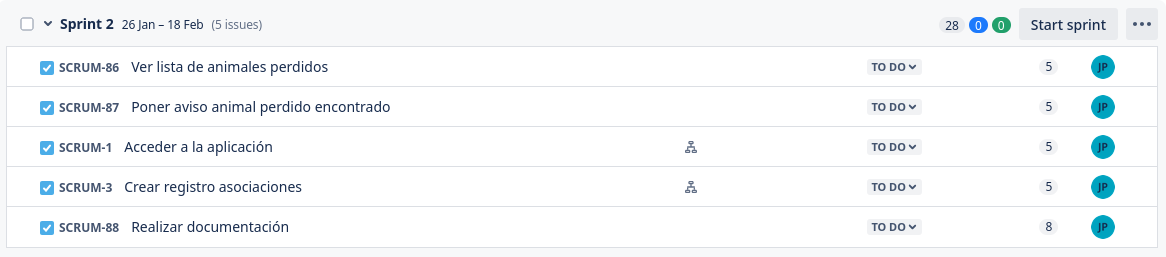
\includegraphics[width=1\linewidth]{newSprint2}
	\caption{Nuevas tareas sprint 2}
	\label{fig:newsprint2}
\end{figure}


Sprint 3 \\
\begin{figure}[H]
	\centering
	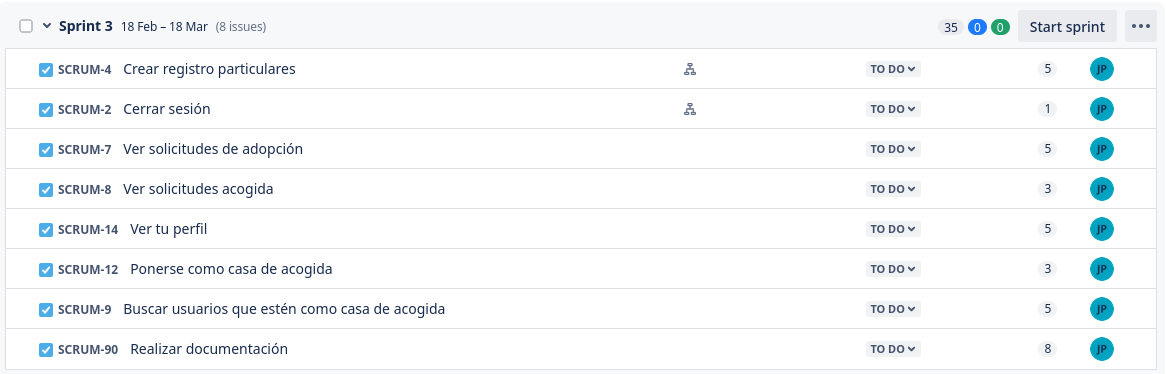
\includegraphics[width=1\linewidth]{newSprint3}
	\caption{Nuevas tareas sprint 3}
	\label{fig:newsprint3}
\end{figure}

Sprint 4 \\
\begin{figure}[H]
	\centering
	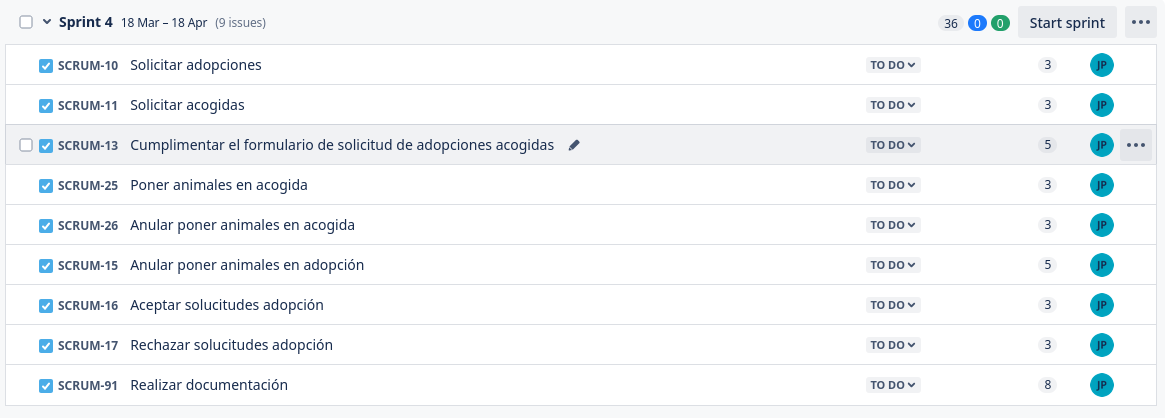
\includegraphics[width=1\linewidth]{newSprint4}
	\caption{Nuevas tareas sprint 4}
	\label{fig:newsprint4}
\end{figure}


Sprint 5 \\ 
\begin{figure}[H]
	\centering
	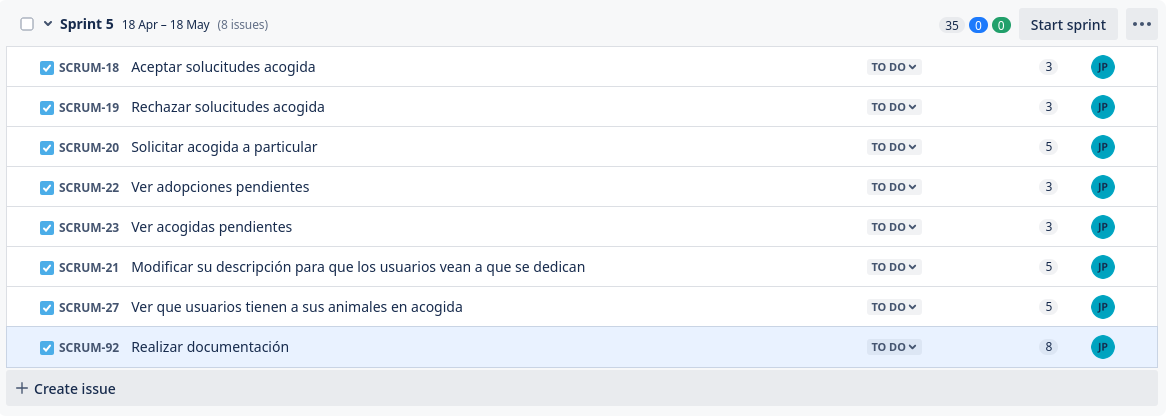
\includegraphics[width=1\linewidth]{newSprint5}
	\caption{Nuevas tareas sprint 5}
	\label{fig:newsprint5}
\end{figure}

El resto de tareas se moverán al backlog para su futura realización. \\ 

\textbf{Backend} \\

Como hemos visto en apartados anteriores (explicar en descripción de la propuesta que uso modelo-vista-controlador) en el back se encuentran tanto los controladores como los modelos para el acceso a la base de datos y su envío a la aplicación móvil. \\

En la finalización del primer sprint la estructura de directorios es la siguiente:

\begin{figure}[H]
	\centering
	\includegraphics[width=0.7\linewidth]{"sprint 1/directoriosBack"}
	\caption{Estructura de directorios del backend al final del sprint 1}
	\label{fig:directoriosback1}
\end{figure}

Además al utilizar un ORM se accede a la base de datos mediante clases por lo que para ilustrar su estructura se ha realizado un diagrama con sus relaciones y funciones básicas:

\begin{figure}[H]
	\centering
	\includegraphics[width=1\linewidth]{"sprint 1/clases"}
	\caption{Diagrama de clases de la primera iteración}
	\label{fig:clases}
\end{figure}


\subsection{Iteración 2}
En esta iteración nos encargaremos tanto de la creación como de la visualización de publicaciones de animales perdidos o encontrados. También crearemos la página de acceso a la aplicación, aunque solo podrán entrar los usuarios particulares ya que son de los únicos que registraremos por ahora, los demás se irán incluyendo en el iteraciones posteriores.  \\

\large{\textbf{Especificación de tareas}} \\

\begin{tabular}{|c|p{9.5cm}|p{1cm}|}
	\hline
	\multicolumn{3}{|c|}{\textbf{HU.3 - Ver lista de animales perdidos/encontrados}} \\
	\hline
	\textbf{Id} & \textbf{Título de la tarea de desarrollo} & \textbf{Est. (días)} \\
	\hline
	3.1 & Realizar bocetos & 0,5 \\ \hline
	3.2 &  Implementar la lógica de acceso a los animales perdidos/encontrados& 2 \\ \hline
	3.3 &  Implementar la interfaz obtener la lista de publicaciones de animales perdidos encontrados& 1 \\ \hline
	3.4 & Crear tabla de publicaciones de animales perdidos/encontrados y tabla de imágenes para dichas publicaciones & 0,5\\ \hline
	\multicolumn{3}{|c|}{\textbf{Pruebas de aceptación}} \\ \hline
	1 & \multicolumn{2}{|p{10cm}|}{Mostrar mensaje en caso de que no haya animales perdidos/encontrados} \\ \hline
	2 & \multicolumn{2}{|p{10cm}|}{Mostrar lista de todos los animales perdidos/encontrados} \\ \hline
	3 & \multicolumn{2}{|p{10cm}|}{Que los filtros de búsqueda funcionen correctamente} \\ \hline
\end{tabular} \\ \\


\begin{tabular}{|c|p{9.5cm}|p{1cm}|}
	\hline
	\multicolumn{3}{|c|}{\textbf{HU.4 - Añadir publicación de animal perdido o encontrado}} \\
	\hline
	\textbf{Id} & \textbf{Título de la tarea de desarrollo} & \textbf{Est. (días)} \\
	\hline
	4.1 & Realizar bocetos & 0,5 \\ \hline
	4.2 &  Actualizar la lógica para añadir publicaciones de perdido o encontrado a la base de datos & 2 \\ \hline
	4.3 &  Implementar la interfaz para crear la publicación de animal perdido/encontrado & 1 \\ \hline
	4.4 &  Implementar la funcionalidad de añadir imágenes a las publicaciones de animal perdido/encontrado & 0,5 \\ \hline
	\multicolumn{3}{|c|}{\textbf{Pruebas de aceptación}} \\ \hline
	1 & \multicolumn{2}{|p{10cm}|}{Comprobar que los campos deben estar cumplimentados antes de realizar la petición de creación al servidor} \\ \hline
	2 & \multicolumn{2}{|p{10cm}|}{Que las imágenes seleccionadas se almacenan apropiadamente} \\ \hline
	3 & \multicolumn{2}{|p{10cm}|}{Que la cámara funcione correctamente en dispositivos móviles} \\ \hline
\end{tabular} \\ \\

\begin{tabular}{|c|p{9.5cm}|p{1cm}|}
	\hline
	\multicolumn{3}{|c|}{\textbf{HU.5 - Crear registro de particulares}} \\
	\hline
	\textbf{Id} & \textbf{Título de la tarea de desarrollo} & \textbf{Est. (días)} \\
	\hline
	5.1 & Realizar bocetos & 0,5 \\ \hline
	5.2 &  Implementar la lógica de registro & 2 \\ \hline
	5.3 &  Implementar la interfaz de registro & 1 \\ \hline
	5.4 &  Implementar la funcionalidad de añadir imágenes de perfil & 0,5 \\ \hline
	\multicolumn{3}{|c|}{\textbf{Pruebas de aceptación}} \\ \hline
	1 & \multicolumn{2}{|p{10cm}|}{Comprobar que los campos deben estar cumplimentados correctamente antes de realizar la petición al servidor} \\ \hline
	2 & \multicolumn{2}{|p{10cm}|}{Asegurarse de que la imágenes seleccionadas se almacena apropiadamente} \\ \hline
	3 & \multicolumn{2}{|p{10cm}|}{Ver que la cámara funcione correctamente en dispositivos móviles} \\ \hline
	4 & \multicolumn{2}{|p{10cm}|}{Ver que los campos de ubicación se autocompletan correctamente en caso de tener los permisos activados} \\ \hline
\end{tabular} \\ \\\\

\begin{tabular}{|c|p{9.5cm}|p{1cm}|}
	\hline
	\multicolumn{3}{|c|}{\textbf{HU.6 - Acceder a la aplicación}} \\
	\hline
	\textbf{Id} & \textbf{Título de la tarea de desarrollo} & \textbf{Est. (días)} \\
	\hline
		6.1 & Realizar bocetos & 0,5 \\ \hline
	6.2 &  Implementar la lógica asociada al inicio de sesión & 2 \\ \hline
	6.3 &  Implementar la interfaz asociada al inicio de sesión de las asociaciones y particulares. & 1,5 \\ \hline
	\multicolumn{3}{|c|}{\textbf{Pruebas de aceptación}} \\ \hline
	1 & \multicolumn{2}{|p{10cm}|}{Comprobar que se avise al usuario si los datos de acceso son incorrectos} \\ \hline
	2 & \multicolumn{2}{|p{10cm}|}{Ver que se envía al usuario a la página principal en caso de que el acceso sea correcto} \\ \hline
	
\end{tabular} \\ \\

\Large{\textbf{HU.3 - Ver lista de animales perdidos/encontrados}} \\

En esta historia nos encargamos de la visualización de las publicaciones sobre animales perdidos que hayan subido los distintos usuarios filtrando como en la HU.1~\pageref{sec:hu1} por diversos filtros para hacer más eficiente la búsqueda.

\textbf{Bocetos}

\begin{figure}[h]
	\centering
	\includegraphics[width=0.31\linewidth]{"sprint 2/hu3/listaPerdidos"}
	\caption{Boceto de la página que lista los animales perdidos/encontrados}
	\label{fig:listaperdidos}
\end{figure}

Como podemos ver en la figura \ref{fig:adopciones}, la estructura es la misma que vimos en la página de lista de adopciones, lo cual genera una cohesión en el diseño de la aplicación, haciéndola más intuitiva para el usuario final.

La única diferencia es que en este caso solo hay un único botón de acción que nos llevará a un chat con la persona que ha publicado el anuncio para poder obtener más información o para dar información sobre la perdida de la mascota.

\textbf{Implementación}
\begin{figure}[H]
	\centering
	\includegraphics[width=0.5\linewidth]{"sprint 2/hu3/disenoFinal"}
	\caption{Vista final de la página que muestra la lista de animales perdidos en móviles}
	\label{fig:listaAdop}
\end{figure}

\begin{figure}[H]
	\centering
	\includegraphics[width=0.8\linewidth]{"sprint 2/hu3/disenoFinalWeb"}
	\caption{Vista final de la página que lista a los animales perdidos en web}
	\label{fig:disenofinalweb}
\end{figure}

Como podemos apreciar, no hay una gran diferencia entre el boceto y la implementación final en la aplicación ya que se mantienen los elementos principales. Además se le ha añadido un botón en la esquina inferior derecha que nos llevará a la página  para añadir una publicación de mascota perdida o encontrada, la cual veremos más adelante.\\

En cuanto a la parte del servidor hemos tenido que crear dos tablas nuevas en la base de datos, una para las publicaciones y otra para las imágenes asociadas a las mismas.\\

Además, también se han creado funciones para el acceso a dichas tablas para su correcto tratamiento y envío a la aplicación móvil para que se muestren correctamente en el formato deseado. Para los filtros se ha reutilizado la mayor parte del código de la HU.1 por lo que eso ha permitido hacer más rápido el desarrollo de esta historia.\\ \\

\Large{\textbf{HU.4 - Añadir publicación de animal perdido o encontrado}}

En esta historia nos vamos a encargar de las tareas relacionadas con el añadido de publicaciones a la sección de mascotas perdidas, para ello deberán rellenar un formulario con distinta información del animal. \\ \\
\textbf{Bocetos}
\begin{figure}[H]
	\centering
	\includegraphics[width=0.31\linewidth]{"sprint 2/hu4/postearPerdido"}
	\caption{Boceto de la página para añadir publicaciones de animales perdidos/encontrados}
	\label{fig:postearperdido}
\end{figure}

Como podemos ver, a diferencia de la página en la que las asociaciones pueden añadir animales a su perfil, en esta tenemos información diferente:

\begin{itemize}
	\item \textbf{Tipo de publicación}: Para este apartado tenemos 2 opciones y son que puede que hayamos \textit{encontrado} un animal en la calle y lo publiquemos en la aplicación para buscar a su dueño, o por el contrario, hemos perdido a nuestra mascota y queremos encontrarla, en este caso sería una publicación del tipo \textit{perdido}. \\ 
	
	\item \textbf{Campos de ubicación}: Éstos los usaremos para identificar el lugar en el que hemos perdido o encontrado al animal en cuestión. Además ayudarán a la posterior consulta de los mismos gracias a la utilización de los filtros en la página de lista de animales perdidos. \\
	
\end{itemize}

\textbf{Implementación}

\begin{figure}[H]
	\centering
	\includegraphics[width=0.8\linewidth]{"sprint 2/hu4/impPerdidos"}
	\caption{Vista final de la página para añadir animales perdidos/encontrados en móviles}
	\label{fig:impperdidos}
\end{figure}

\begin{figure}[H]
	\centering
	\includegraphics[width=0.8\linewidth]{"sprint 2/hu4/impPerdidosWeb"}
	\caption{Vista final de la página para añadir animales perdidos/encontrados en web}
	\label{fig:impperdidosweb}
\end{figure}

Como podemos ver en la implementación para móviles, en función del tipo de publicación que sea (perdido o encontrado), la información que rellena el usuario es ligeramente diferente, ya que por ejemplo alguien que haya encontrado un perro perdido no va a saber su nombre como sí lo haría el dueño del animal. El otro campo es la zona de desaparición para el caso de perder a tu mascota, que sería el lugar de de recogida para el que lo encuentre y/o la zona en la que se halle ahora mismo. \\

Además, en esta historia cabe destacar que se soluciona un problema existente en las imágenes. Antes se podían subir imágenes de cualquier tamaño a la aplicación, haciendo que el ancho y el alto de las publicaciones pudiera llegar a ser diferentes, ahora todas deben tener el mismo ratio de escala, para que así cuando se visualicen todas las publicaciones, éstas tengan el mismo tamaño, haciendo del diseño algo más consistente.\\

En el frontend hemos añadido la librería \textit{ngx-image-cropper} \cite{cropper}, la cual nos permite recortar las imágenes con un ratio determinado, como se ha mencionado anteriormente, lo que ha acelerado el desarrollo de la historia. El funcionamiento es sencillo, cada vez que subimos una imagen se nos pedirá que la recortemos con la proporción adecuada, pudiendo mover el selector por la imagen y haciéndola más grande o más pequeña en función de nuestras necesidades. \\

En cuanto a la base de datos, gracias a la historia anterior no debemos añadir ninguna tabla más. Por otra parte hemos creado un endpoint del tipo \textit{POST}, esto es un punto de acceso en el servidor para recibir peticiones del cliente, para añadir publicaciones a la base de datos. \\

También hemos creado una función para añadir la publicación, y para agregar las imágenes, hemos reutilizado la creada en la adición de animales en adopción, con unos pequeños cambios, como cambiar la ruta de almacenaje de las imágenes. \\ 




\Large{\textbf{HU.5 - Crear registro de particulares}}

Esta historia, como su título nos indica comprende la creación de una página para el registro de usuarios, se trata de un formulario con la información pertinente para su correcta gestión.\\

\textbf{Bocetos}
\begin{figure}[H]
	\centering
	\includegraphics[width=0.31\linewidth]{"sprint 2/hu5/registro_particulares"}
	\caption{Boceto de la página de registro de particulares}
	\label{fig:registroparticulares}
\end{figure}

La estructura básica de la página es simple, tenemos un conjunto de campos a cubrir y un botón el cual nos permitirá enviar la información al servidor para realizar la creación del mismo. \\

\textbf{Implementación}

\begin{figure}[H]
	\centering
	\includegraphics[width=0.7\linewidth]{"sprint 2/hu5/impRegistroParticulares"}
	\caption{Vista final de la página de creación de particulares en móviles}
	\label{fig:impregistroparticulares}
\end{figure}

\begin{figure}[H]
	\centering
	\includegraphics[width=0.7\linewidth]{"sprint 2/hu5/impRegistroParticularesWeb"}
	\caption{Vista final de la página de creación de particulares en Web}
	\label{fig:impregistroparticularesweb}
\end{figure}


Como vemos para la parte del frontend, no hay demasiada diferencia con los bocetos en la implementación final. Lo que sí que podemos observar es que a diferencia de los otros formularios, en el tema claro los elementos tienen un fondo grisáceo asemejándose así al tema oscuro. Cabe destacar que este cambio ha sido aplicado al resto de formularios de forma retroactiva. Esto se ha decidido para hacer más homogénea la aplicación.

Además, en cuanto al apartado de diseño también se ha ajustado el ancho en la versión web, para que los elementos no ocupen todo el ancho de la página.

En cuanto a la programación, debemos destacar los siguientes aspectos:

\begin{itemize}
	\item \textbf{Obtención dinámica de localización}: Para esta historia se ha implementado la geolocalización, lo que nos permite acceder a la ubicación del dispositivo y así autocompletar la información referente a la ubicación sin que el usuario tenga que hacer nada. Para ello hemos hecho uso de la librería \textit{opencage-api-client}, la cual nos devuelve información sobre la localización actual del dispositivo. En este caso utilizamos la provincia, y desde ella obtenemos el país al cual pertenece en nuestra base de datos. 
	
	En el servidor se han creado funciones para la obtención dinámica de la ubicación, para ello éste recibe la provincia del cliente y de ella obtiene el país al que pertenece y se retorna a la aplicación un estructura con todos los países y sus provincias, la provincia actual y el país al que pertenece, esto es lo que en el frontend nos permite rellenar los selectores correctamente.
	
	En caso de no tener activada la geolocalización, el usuario debe introducirlo manualmente, si no la aplicación le avisará de un error.
	
	Esto se ha implementado también en la página de publicar animales perdidos por motivos prácticos.
	
	
	\item \textbf{Control de errores}: En caso de que el usuario se deje alguno de los campos obligatorios sin rellenar cuando pulse el botón de crear cuenta, se le avisará mediante un \textit{toast}, esto es una alerta temporal que aparece en la parte inferior de la pantalla. En este caso todos los campos son obligatorios, a excepción de la fotografía.
	
	Además, también en el momento de la inserción se comprueba previamente si tanto el correo como el nombre de usuario están en uso actualmente, y, en caso de estarlo, se le notificará al usuario que alguno de éstos ya está en uso.
\end{itemize}

Se ha creado un endpoint para la información que tenga que ver con los usuarios, en este caso su creación y la comprobación de que el usuario a registrar en la aplicación no exista actualmente.

Un detalle a comentar sobre la estructura de la base de datos es que en el diagrama de la iteración 1 los usuarios no tenían el campo de contraseña, este ya se ha añadido, como se reflejará en el diagrama al final de esta iteración. \\


\Large{\textbf{HU.6 - Acceder a la aplicación}} 

En el desarrollo de esta historia hemos realizado la creación de la página de \textit{log in} para que los distintos usuarios puedan acceder a la misma y acceder a contenido limitado o específico de un tipo de usuario concreto. \\ 

\textbf{Bocetos}


\begin{figure}[H]
	\centering
	\includegraphics[width=0.31\linewidth]{"sprint 2/hu6/login"}
	\caption{Boceto de la pantalla de acceso}
	\label{fig:login}
\end{figure}

Como podemos apreciar en el boceto la página, ésta contará con un pequeño formulario de inicio de sesión en el cual se deberá rellenar con el nombre de usuario y su contraseña pertinente. Además también vemos que desde esta página se podrá ir a la de registro (Crear cuenta), en el caso de no estar registrado previamente. \\

\textbf{Implementación}

\begin{figure}[H]
	\centering
	\includegraphics[width=0.7\linewidth]{"sprint 2/hu6/ImpLoginMovil"}
	\caption{Diseño final de la página de acceso en móviles}
	\label{fig:imploginmovil}
\end{figure}

\begin{figure}[H]
	\centering
	\includegraphics[width=0.7\linewidth]{"sprint 2/hu6/ImpLoginWeb"}
	\caption{Diseño final de la página de acceso en web}
	\label{fig:imploginweb}
\end{figure}

Como podemos ver en el diseño final, no ha habido cambios significativos con respecto a los bocetos, pero si que se ha cambiado la estética en los botones de la aplicación ahora son más redondeados, esto se ha hecho con carácter retroactivo aplicándose al resto de páginas. El motivo ha sido hacer una interfaz más acorde a las corrientes actuales.

En esta página hemos creado un pequeño formulario con los datos de inicio de sesión que se enviarán al servidor en cuanto le demos aceptar.

Si se hayan fallos en las credenciales, se le notificará al usuario que ha habido un error, si son correctas se accederá de manera normal a la aplicación.

Para mantener al usuario conectado hemos hecho uso sesiones. Para esto hemos instalado la librería \textit{express-session} la cual nos permite almacenar los datos que necesitemos para mantener las sesiones de los usuarios, además de enviar una \textit{cookie} con el id de la sesión al usuario, lo que nos permitirá acceder a su información cuando se hagan peticiones al servidor.

Hemos creado un endpoint para el \textit{login (/api/login)} en el cual tenemos 2 métodos, uno para comprobar si las credenciales son correctas y otro para saber si el usuario tiene ya una sesión activa. En el primero debemos asegurarnos de crear la sesión y enviarle la cookie a la aplicación.

Con todo esto ya tenemos terminada la lógica del acceso en el servidor, pero también hemos tenido que controlar el acceso a las páginas de la aplicación a las que no se puede acceder si no estás "logueado", y hacer que aparezcan o no ciertos elementos en función del tipo de usuario que esté conectado. Esto además se irá actualizando con el tiempo a medida que se vayan creando nuevas páginas. \\

\Large{\textbf{Fin del sprint}} \\

La estructura actual de directorios en el backend es la siguiente: 

\begin{figure}[H]
	\centering
	\includegraphics[width=0.7\linewidth]{"sprint 2/directoriosBackS2"}
	\caption{Estructura de directorios del backend al final del sprint}
	\label{fig:directoriosbacks2}
\end{figure}

Además también se ha actualizado el diagrama de clases, ya que aunque en esta iteración no se han creado nuevas clases se han realizado otros cambios, como añadir los métodos necesarios para la búsqueda de país a partir de una provincia o los asociados a la creación de usuarios.

\begin{figure}[H]
	\centering
	\includegraphics[width=1\linewidth]{"sprint 2/clases"}
	\caption{Diagrama de clases de la segunda iteración}
	\label{fig:clases2}
\end{figure}


Como cierre de la iteración a nivel de tareas se han realizado todas las HU propuestas. No obstante, la realización de pruebas y corrección de este documento ha abarcado más de lo esperado ocupando 4 días del siguiente sprint.

\subsection{Iteración 3}
En esta iteración crearemos el registro de asociaciones crearemos una página para recibir solicitudes de adopción y/o acogida, crearemos la página para ver nuestro perfil, haremos que los usuarios particulares puedan ponerse como casa de acogida, para que las asociaciones los puedan buscar y pedirles que acojan a alguno de sus animales. Por último también mejoraremos el uso de sesiones haciéndolas persistentes frente a caídas del servidor. \\ \\
\textbf{Especificación de tareas} \\

\begin{tabular}{|c|p{9.5cm}|p{1cm}|}
	\hline
	\multicolumn{3}{|c|}{\textbf{HU.7 - Cerrar sesión}} \\
	\hline
	\textbf{Id} & \textbf{Título de la tarea de desarrollo} & \textbf{Est. (días)} \\
	\hline
	7.1 & Realizar de bocetos. & 0,5 \\ \hline
	7.2 &  Implementar la lógica asociada al cierre de sesión. & 1 \\ \hline
	7.3 &  Implementar interfaz asociada al cierre de sesión. & 0.5 \\ \hline
	\multicolumn{3}{|c|}{\textbf{Pruebas de aceptación}} \\ \hline
	1 & \multicolumn{2}{|p{10cm}|}{Comprobar que una vez cerrada la sesión el usuario no pueda acceder a páginas restringidas.} \\ \hline
\end{tabular} \\ \\

\begin{tabular}{|c|p{9.5cm}|p{1cm}|}
	\hline
	\multicolumn{3}{|c|}{\textbf{HU.8 - Crear registro de asociaciones}} \\
	\hline
	\textbf{Id} & \textbf{Título de la tarea de desarrollo} & \textbf{Est. (días)} \\
	\hline
	8.1 & Realizar bocetos. & 0,5 \\ \hline
	8.2 &  Implementar la lógica de registro. & 2 \\ \hline
	8.3 &  Implementar la interfaz de registro. & 1 \\ \hline
	8.4 &  Implementar la funcionalidad de añadir imágenes de perfil. & 0,5 \\ \hline
	8.5 &  Encriptar el archivo del acta fundacional. & 0,5 \\ \hline
	
	\multicolumn{3}{|c|}{\textbf{Pruebas de aceptación}} \\ \hline
	1 & \multicolumn{2}{|p{10cm}|}{Comprobar que los campos deben estar cumplimentados correctamente antes de realizar la petición al servidor.} \\ \hline
	2 & \multicolumn{2}{|p{10cm}|}{Asegurarse de que la imágenes seleccionadas se almacenan apropiadamente.} \\ \hline
	3 & \multicolumn{2}{|p{10cm}|}{Ver que la cámara funcione correctamente en dispositivos móviles.} \\ \hline
	4 & \multicolumn{2}{|p{10cm}|}{Ver que los campos de ubicación se autocompletan correctamente en caso de tener los permisos activados.} \\ \hline
	5 & \multicolumn{2}{|p{10cm}|}{Comprobar que el archivo se encripta correctamente.} \\ \hline
	
\end{tabular} \\ \\

\begin{tabular}{|c|p{9.5cm}|p{1cm}|}
	\hline
	\multicolumn{3}{|c|}{\textbf{HU.9 - Ver solicitudes de adopción}} \\
	\hline
	\textbf{Id} & \textbf{Título de la tarea de desarrollo} & \textbf{Est. (días)} \\
	\hline
	9.1 & Realizar bocetos. & 0,5 \\ \hline
	9.2 &  Implementar la lógica. & 2 \\ \hline
	9.3 &  Implementar la interfaz para la visualización. & 1 \\ \hline
	9.4 &  Crear tabla de solicitudes & 0,5 \\ \hline
	\multicolumn{3}{|c|}{\textbf{Pruebas de aceptación}} \\ \hline
	1 & \multicolumn{2}{|p{10cm}|}{Comprobar que las solicitudes se envían correctamente.} \\ \hline
	2 & \multicolumn{2}{|p{10cm}|}{Comprobar que las asociaciones no puedan hacer peticiones de adopción.} \\ \hline
	3 & \multicolumn{2}{|p{10cm}|}{Comprobar que a un usuario no registrado se le avise de que no puede adoptar en caso de intentarlo.} \\ \hline
	4 & \multicolumn{2}{|p{10cm}|}{Comprobar que no se guardan solicitudes de adopción/acogida repetidas.} \\ \hline
	
	
\end{tabular} \\ \\

\begin{tabular}{|c|p{9.5cm}|p{1cm}|}
	\hline
	\multicolumn{3}{|c|}{\textbf{HU.10 - Ver solicitudes de acogida}} \\
	\hline
	\textbf{Id} & \textbf{Título de la tarea de desarrollo} & \textbf{Est. (días)} \\
	\hline
	10.1 & Realizar bocetos. & 0,5 \\ \hline
	10.2 &  Implementar la lógica. & 1 \\ \hline
	10.3 &  Implementar la interfaz para la visualización. & 1 \\ \hline
	\multicolumn{3}{|c|}{\textbf{Pruebas de aceptación}} \\ \hline
	1 & \multicolumn{2}{|p{10cm}|}{Comprobar que las solicitudes se envían correctamente.} \\ \hline
	2 & \multicolumn{2}{|p{10cm}|}{Comprobar que las asociaciones no puedan hacer peticiones de acogida.} \\ \hline
	3 & \multicolumn{2}{|p{10cm}|}{Comprobar que a un usuario no registrado se le avise de que no puede acoger en caso de intentarlo.} \\ \hline
	4 & \multicolumn{2}{|p{10cm}|}{Comprobar que a un usuario no registrado se le avise de que no puede adoptar en caso de intentarlo.} \\ \hline
	5 & \multicolumn{2}{|p{10cm}|}{Comprobar que no se guardan notificaciones repetidas.} \\ \hline
	
\end{tabular} \\ \\

\begin{tabular}{|c|p{9.5cm}|p{1cm}|}
	\hline
	\multicolumn{3}{|c|}{\textbf{HU.11 - Ver tu perfil}} \\
	\hline
	\textbf{Id} & \textbf{Título de la tarea de desarrollo} & \textbf{Est. (días)} \\
	\hline
	11.1 & Realizar bocetos & 0,5 \\ \hline
	11.2 &  Implementar la lógica de obtención del perfil & 2 \\ \hline
	11.3 &  Implementar la interfaz para la visualización del perfil & 1 \\ \hline
	\multicolumn{3}{|c|}{\textbf{Pruebas de aceptación}} \\ \hline
	1 & \multicolumn{2}{|p{10cm}|}{Comprobar que los datos obtenidos sean correctos} \\ \hline
	
\end{tabular} \\ \\

\begin{tabular}{|c|p{9.5cm}|p{1cm}|}
	\hline
	\multicolumn{3}{|c|}{\textbf{HU.12 - Ponerse como casa de acogida}} \\
	\hline
	\textbf{Id} & \textbf{Título de la tarea de desarrollo} & \textbf{Est. (días)} \\
	\hline
	12.1 & Realizar bocetos & 0,5 \\ \hline
	12.2 &  Implementar la lógica & 2 \\ \hline
	12.3 &  Implementar la interfaz & 1 \\ \hline
	\multicolumn{3}{|c|}{\textbf{Pruebas de aceptación}} \\ \hline
	1 & \multicolumn{2}{|p{10cm}|}{Ver que el usuario particular sea el único que pueda acceder a esta opción} \\ \hline
	2 & \multicolumn{2}{|p{10cm}|}{Comprobar que los datos son actualizados correctamente en la base de datos} \\ \hline
	
\end{tabular} \\ \\

\begin{tabular}{|c|p{9.5cm}|p{1cm}|}
	\hline
	\multicolumn{3}{|c|}{\textbf{HU.13 - Buscar particulares que estén como casa de acogida}} \\
	\hline
	\textbf{Id} & \textbf{Título de la tarea de desarrollo} & \textbf{Est. (días)} \\
	\hline
	13.1 & Realizar bocetos & 0,5 \\ \hline
	13.2 &  Implementar la lógica & 2 \\ \hline
	13.3 &  Implementar la interfaz & 1 \\ \hline
	\multicolumn{3}{|c|}{\textbf{Pruebas de aceptación}} \\ \hline
	1 & \multicolumn{2}{|p{12cm}|}{Que solo aparezcan usuarios particulares que estén como casa de acogida} \\ \hline
	2 & \multicolumn{2}{|p{12cm}|}{Cuando se le envíe a alguien una petición para acoger, éste la reciba correctamente} \\ \hline
	3 & \multicolumn{2}{|p{12cm}|}{Que el filtro para buscar particulares por provincias funcione correctamente} \\ \hline
	
\end{tabular} \\ \\

\begin{tabular}{|c|p{9.5cm}|p{1cm}|}
	\hline
	\multicolumn{3}{|c|}{\textbf{HU.14 - Solicitar Adopciones/Acogidas}} \\
	\hline
	\textbf{Id} & \textbf{Título de la tarea de desarrollo} & \textbf{Est. (días)} \\
	\hline
	14.1 &  Implementar la lógica & 2 \\ \hline
	14.2 &  Implementar funcionalidad en los botones de las publicaciones de las asociaciones para poder solicitar adoptar/acoger & 1 \\ \hline
	\multicolumn{3}{|c|}{\textbf{Pruebas de aceptación}} \\ \hline
	1 & \multicolumn{2}{|p{12cm}|}{En caso de error se le notifique al usuario} \\ \hline
	2 & \multicolumn{2}{|p{12cm}|}{En caso de que sea satisfactoria se le notifique al usuario} \\ \hline
	
\end{tabular} \\ \\

\begin{tabular}{|c|p{9.5cm}|p{1cm}|}
	\hline
	\multicolumn{3}{|c|}{\textbf{HU.15 - Eliminar solicitudes de Adopciones/Acogidas}} \\
	\hline
	\textbf{Id} & \textbf{Título de la tarea de desarrollo} & \textbf{Est. (días)} \\
	\hline
	15.1 & Implementar la lógica & 2 \\ \hline
	15.2 & Implementar la interfaz & 1 \\ \hline 
	\multicolumn{3}{|c|}{\textbf{Pruebas de aceptación}} \\ \hline
	1 & \multicolumn{2}{|p{12cm}|}{Que se muestre el aviso de borrado para confirmarlo} \\ \hline
	2 & \multicolumn{2}{|p{12cm}|}{Cuando se vuelvan a obtener las notificaciones no aparezca la eliminada} \\ \hline
	
\end{tabular} \\ \\

\begin{tabular}{|c|p{9.5cm}|p{1cm}|}
	\hline
	\multicolumn{3}{|c|}{\textbf{HU.16 - Añadir persistencia a las sesiones}} \\
	\hline
	\textbf{Id} & \textbf{Título de la tarea de desarrollo} & \textbf{Est. (días)} \\
	\hline
	16.1 &  Implementar la lógica & 1,5 \\ \hline
	\multicolumn{3}{|c|}{\textbf{Pruebas de aceptación}} \\ \hline
	1 & \multicolumn{2}{|p{12cm}|}{Cuando se reinicie el servidor se siga manteniendo la sesión} \\ \hline
	2 & \multicolumn{2}{|p{12cm}|}{Ver que te deja acceder al login cuando cierras la sesión} \\ \hline
	
\end{tabular} \\ \\

\Large{\textbf{HU.8 - Crear registro de asociaciones}}

\textbf{Bocetos} \\
\begin{figure}[H]
	\centering
	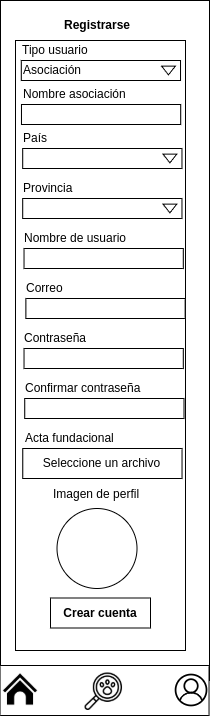
\includegraphics[width=0.31\linewidth]{sprint 3//hu8/registro_asociaciones.png}
	\caption{Boceto del registro de asociaciones}
	\label{fig:boceto_regAso}
\end{figure}

\textbf{Implementación}

\begin{figure} [H]
	\centering
	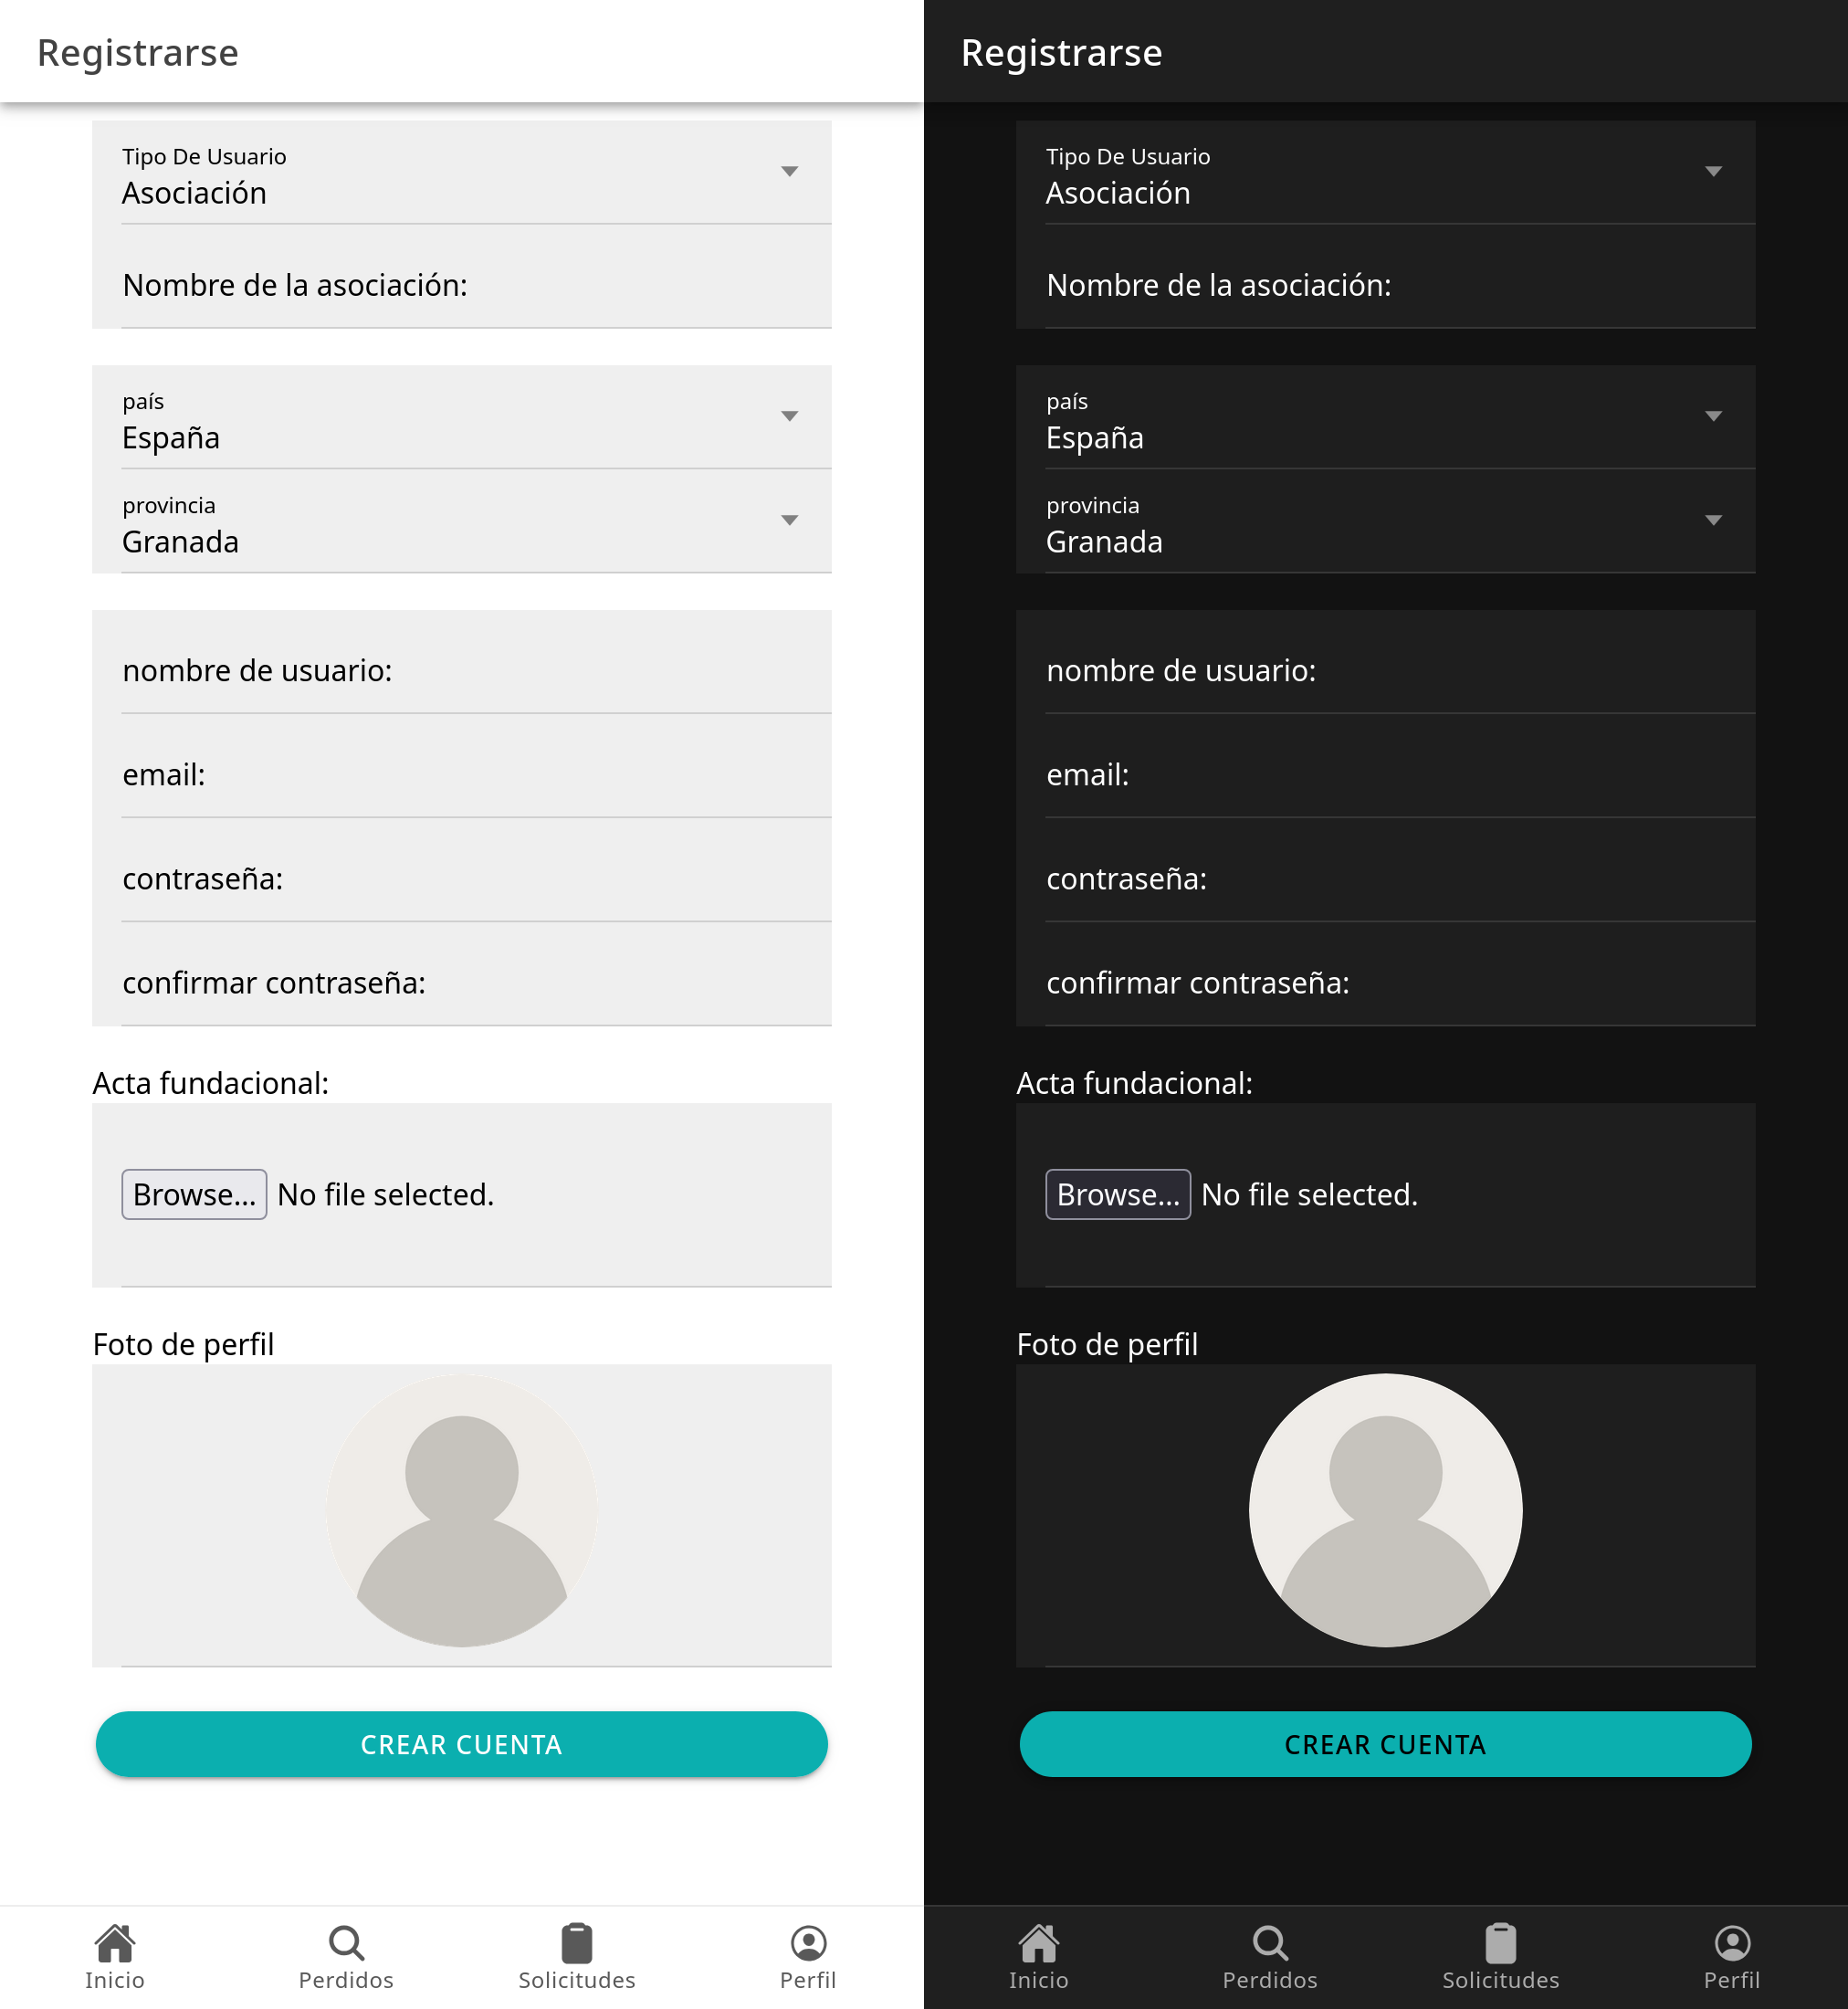
\includegraphics[width=1\linewidth]{sprint 3//hu8/implementacion.png}
	\caption{Diseño del registro de asociaciones en móviles}
	\label{fig:impRegAso}
\end{figure}

\begin{figure}[H]
	\centering
	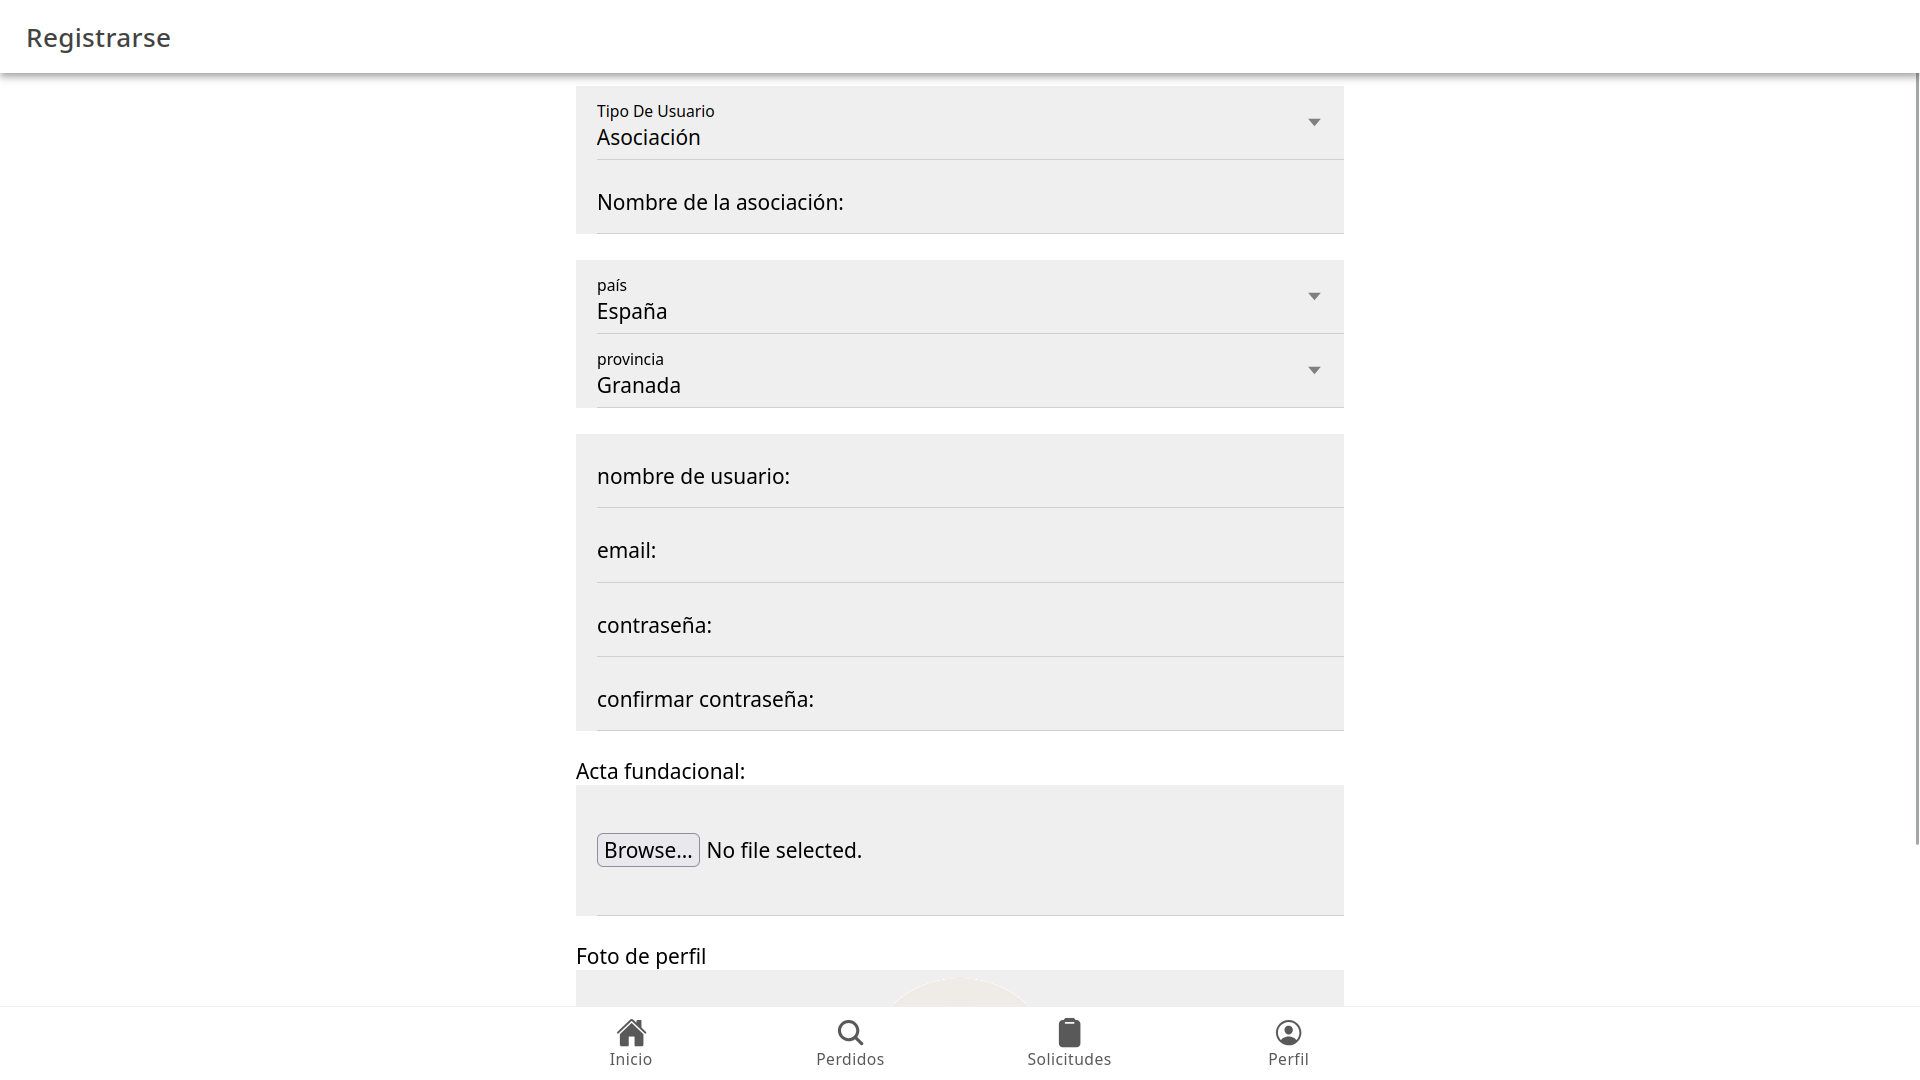
\includegraphics[width=1\linewidth]{sprint 3//hu8/implementacionWeb.png}
	\caption{Diseño del registro de asociaciones en web}
\end{figure}

\Large{\textbf{HU.9 - Ver solicitudes de adopción y HU.10 - Ver solicitudes de acogida}} \\

Para estas historias finalmente se ha decidido juntarlas en una página llamada solicitudes, ya que el código de ambas era muy similar y así evitamos duplicidad de código.

\textbf{Bocetos}
\begin{figure}[H]
	\centering
	\includegraphics[width=0.31\linewidth]{sprint 3//hu9-10/solicitudesAcogidaAdopción.png}
	\caption{Boceto del la página de solicitudes}
	\label{fig:boceto_adopt}
\end{figure}


\textbf{Implementación}

\begin{figure} [H]
	\centering
	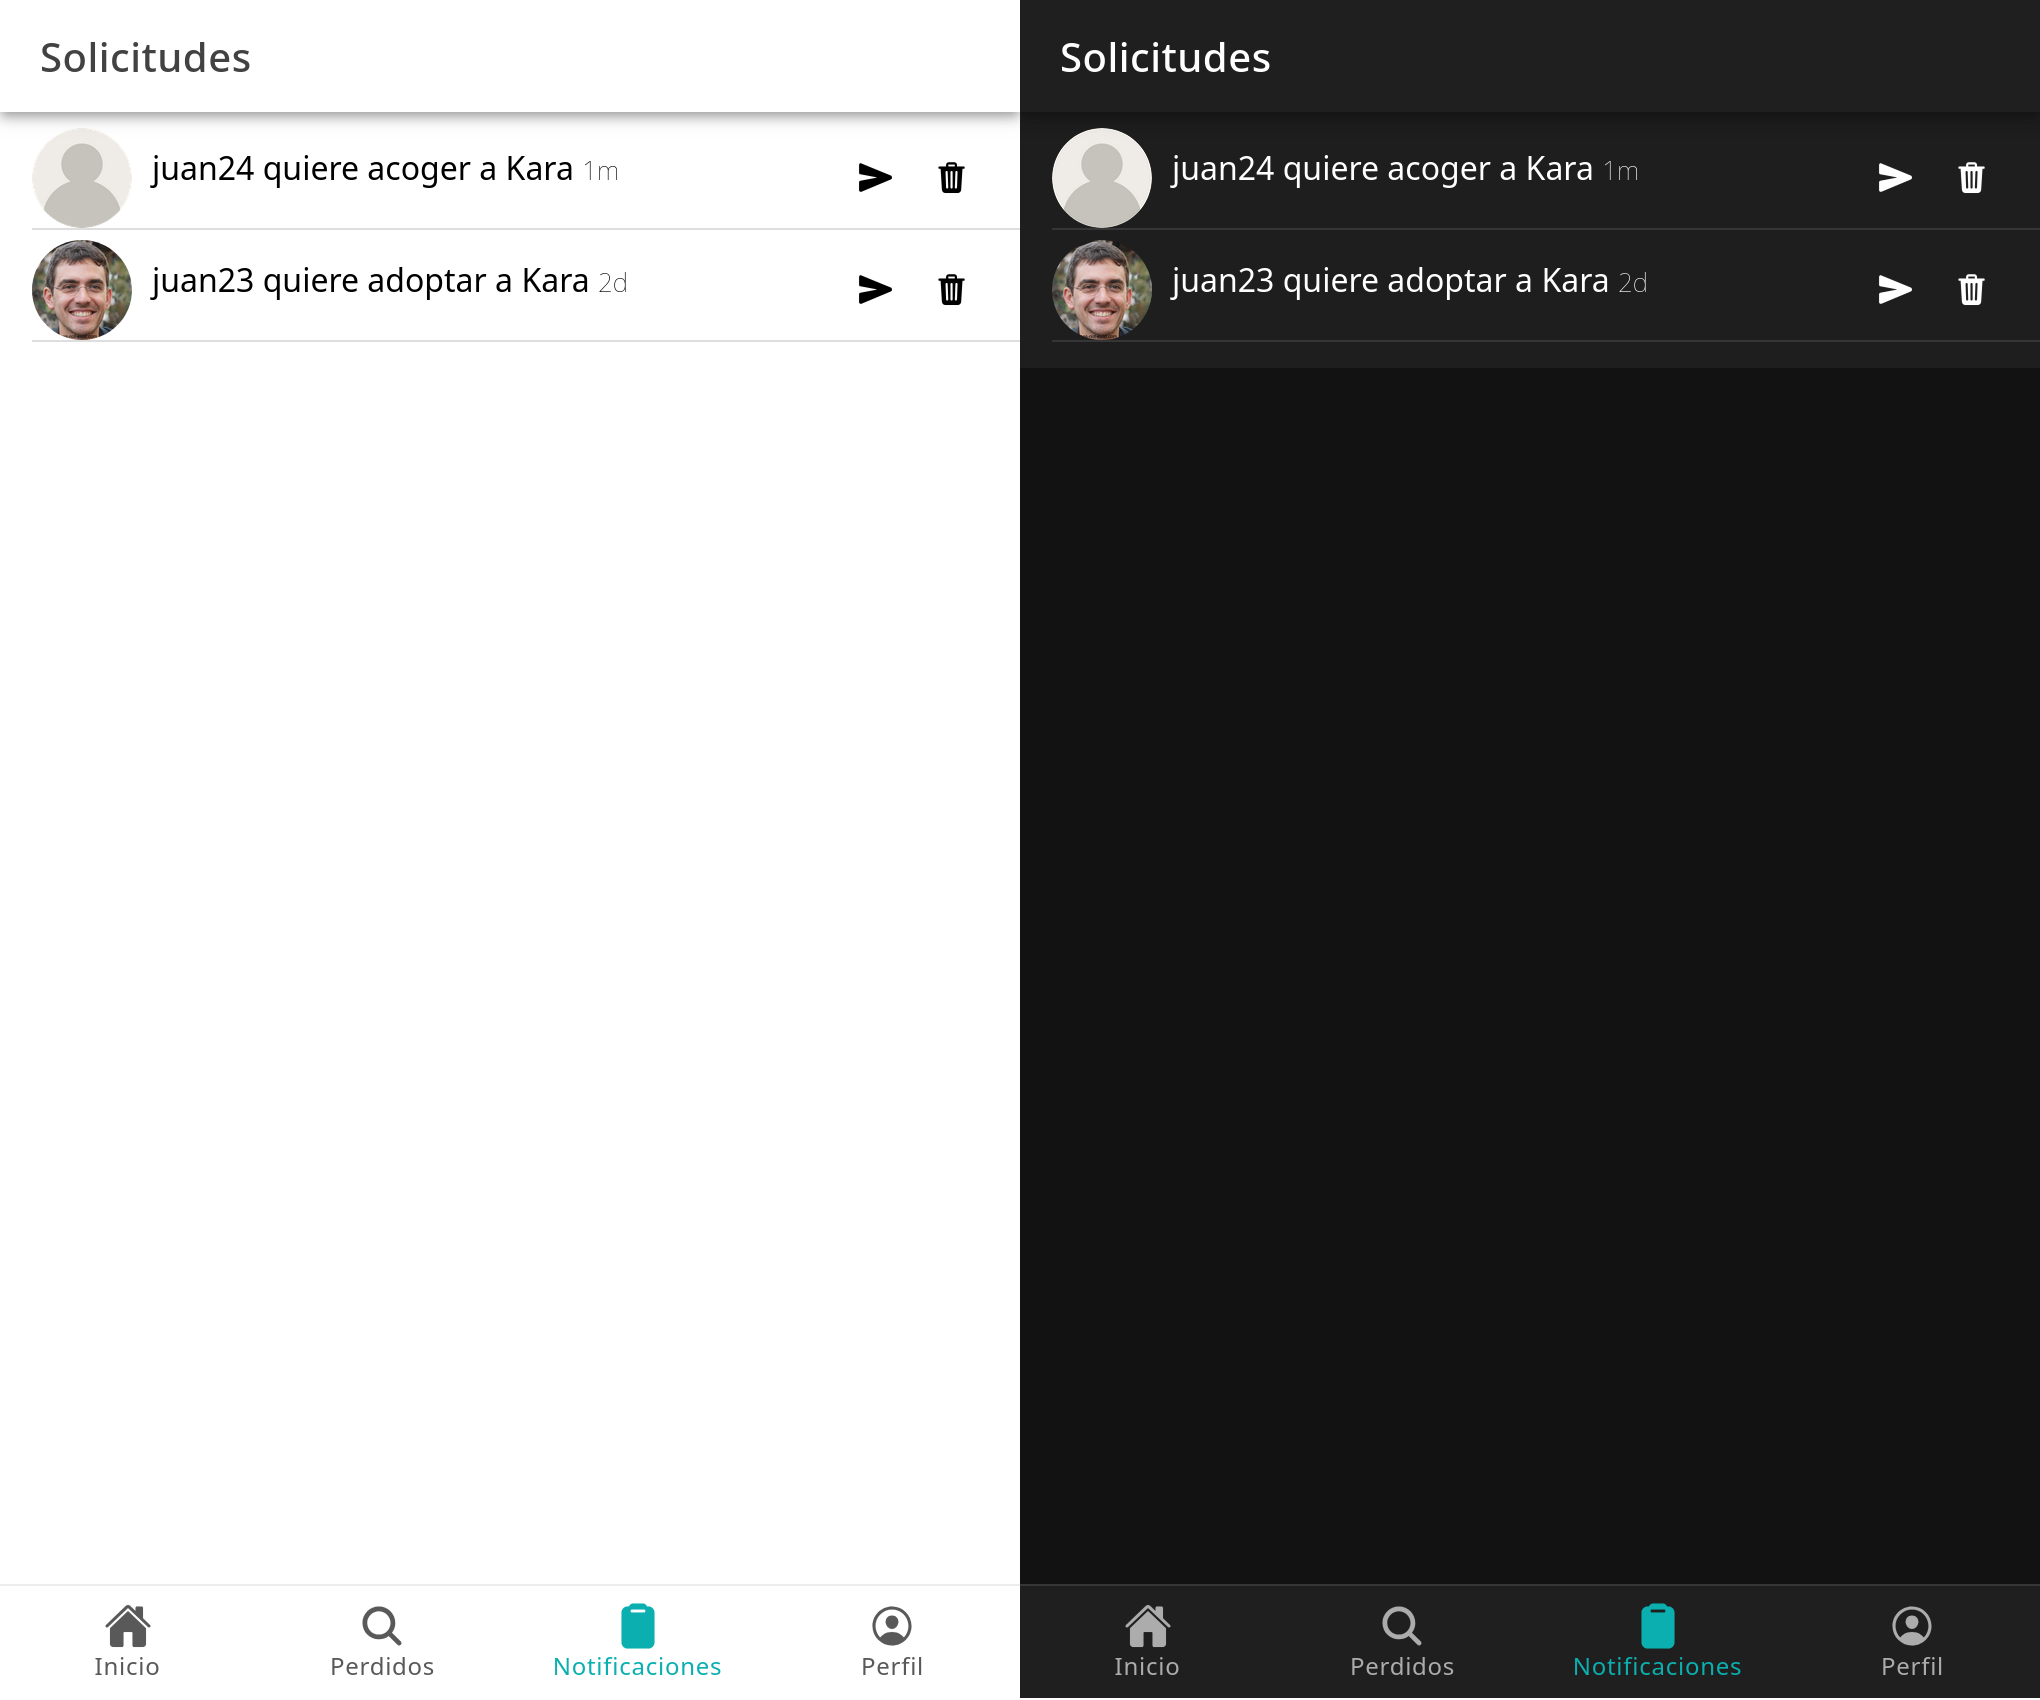
\includegraphics[width=1\linewidth]{sprint 3//hu9-10/solicitudes.png}
	\caption{Diseño de la página de solicitudes de asociaciones en móviles}
	\label{fig:notificaciones}
\end{figure}

\begin{figure}[H]
	\centering
	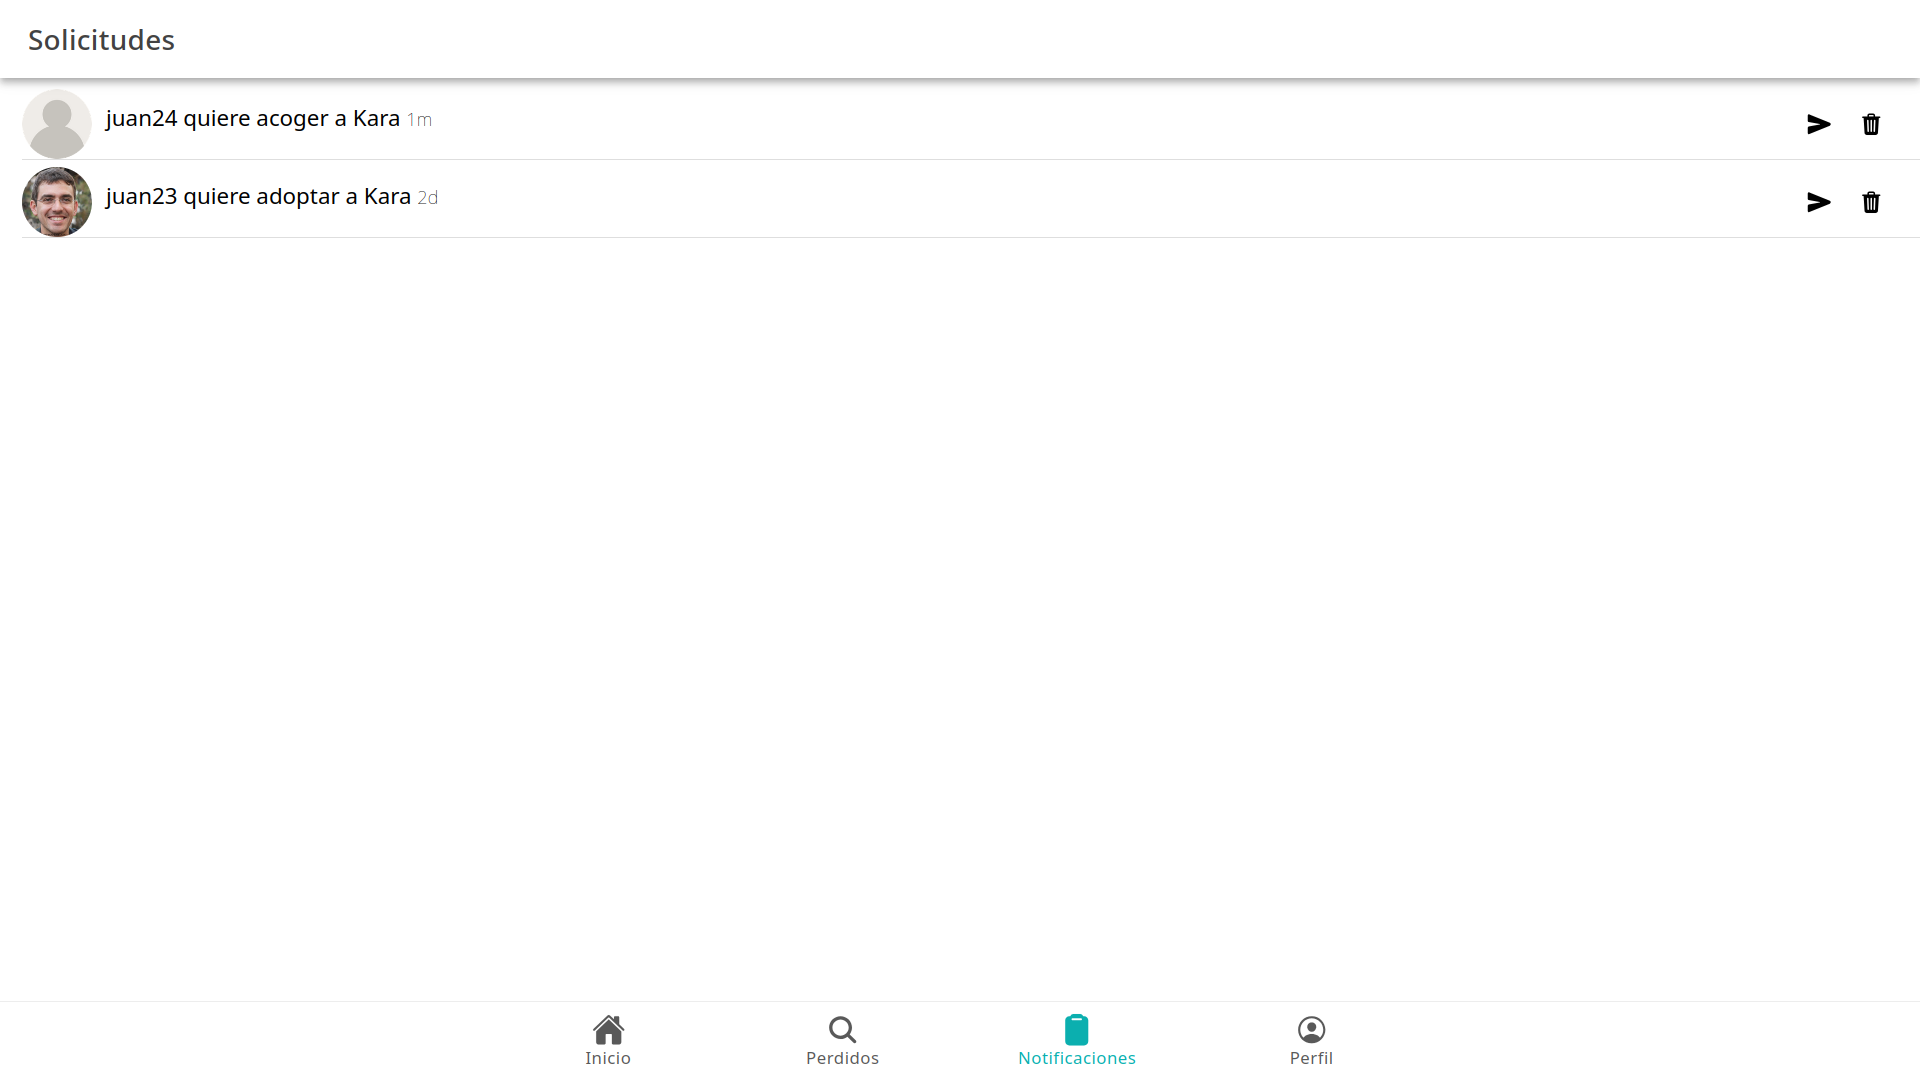
\includegraphics[width=1\linewidth]{sprint 3//hu9-10/solicitudesWeb.png}
	\caption{Diseño de la página de solicitudes de asociaciones en web}
\end{figure}

\Large{\textbf{HU.11 - Ver tu perfil y HU.12 - Ponerse como casa de acogida}} \\

Hemos decidido juntar estas dos historias ya que ponerse como casa de acogida se realiza dentro del perfil del usuario en cuestión.

\textbf{Bocetos} \\
\begin{figure}[H]
	\centering
	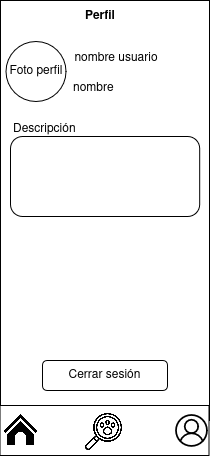
\includegraphics[width=0.31\linewidth]{sprint 3//hu11-12/boceto.png}
	\caption{Boceto de la página del perfil}
\end{figure}

\textbf{Implementación}

\begin{figure} [H]
	\centering
	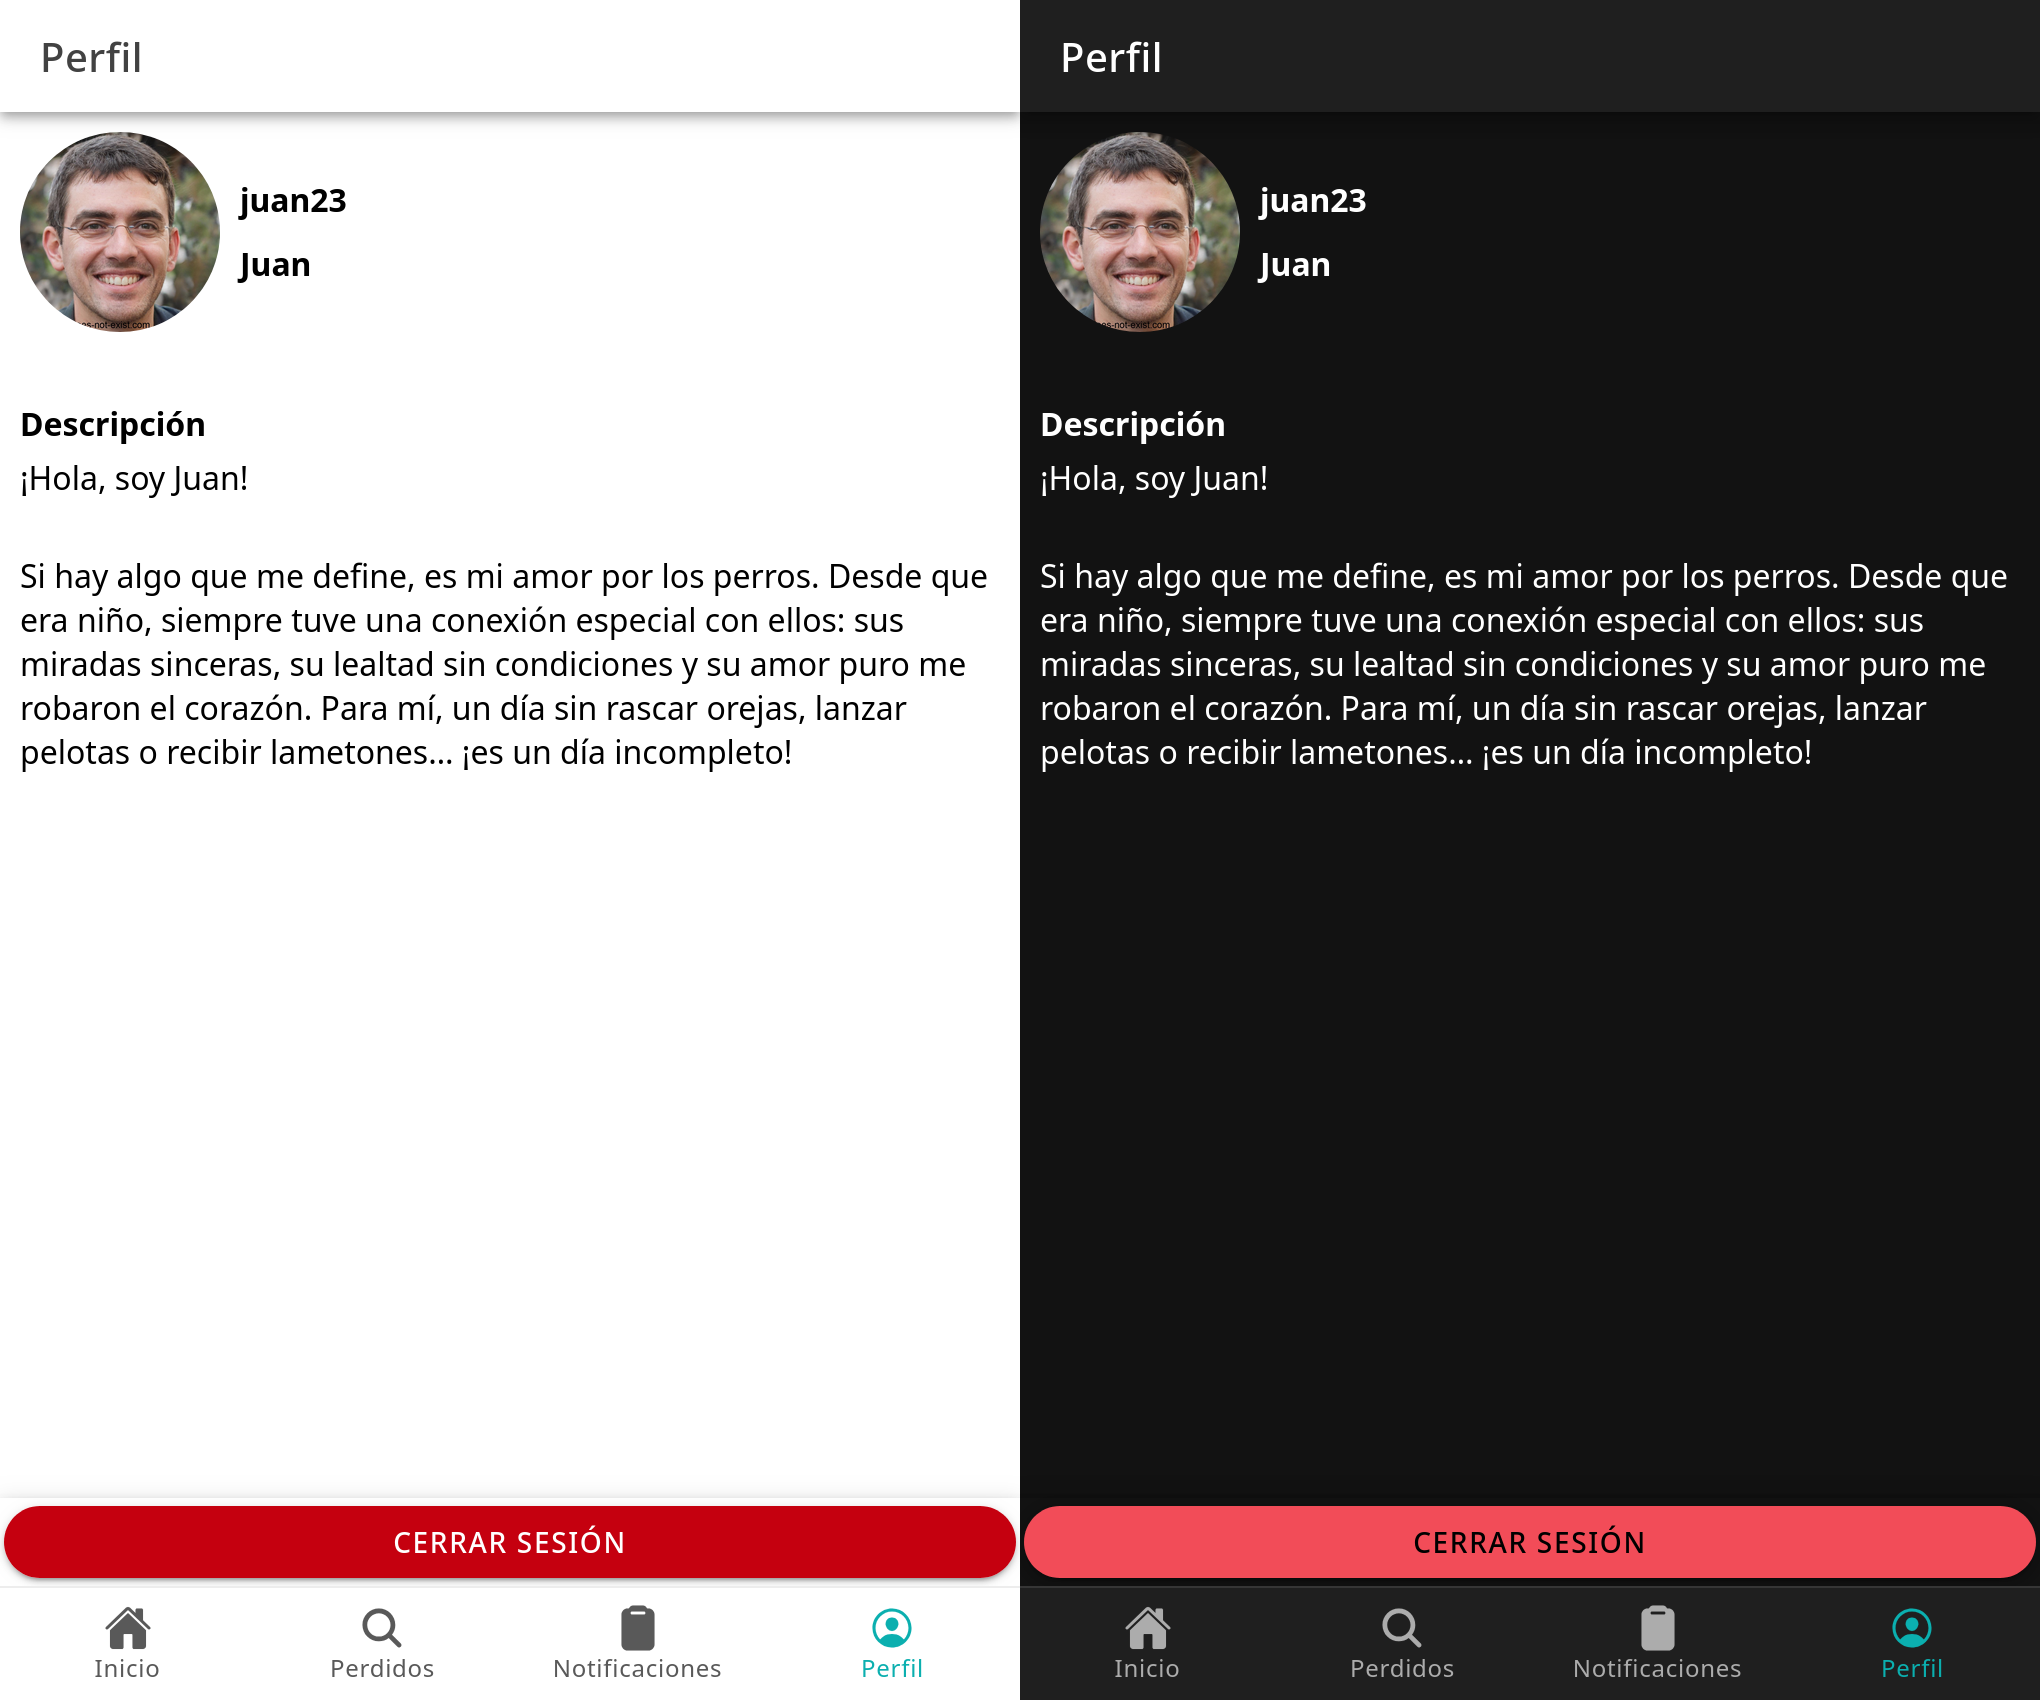
\includegraphics[width=1\linewidth]{sprint 3//hu11-12/implementacion.png}
	\caption{Diseño de la página para ver el perfil en móviles}
	\label{fig:impPerfil}
\end{figure}

\begin{figure}[H]
	\centering
	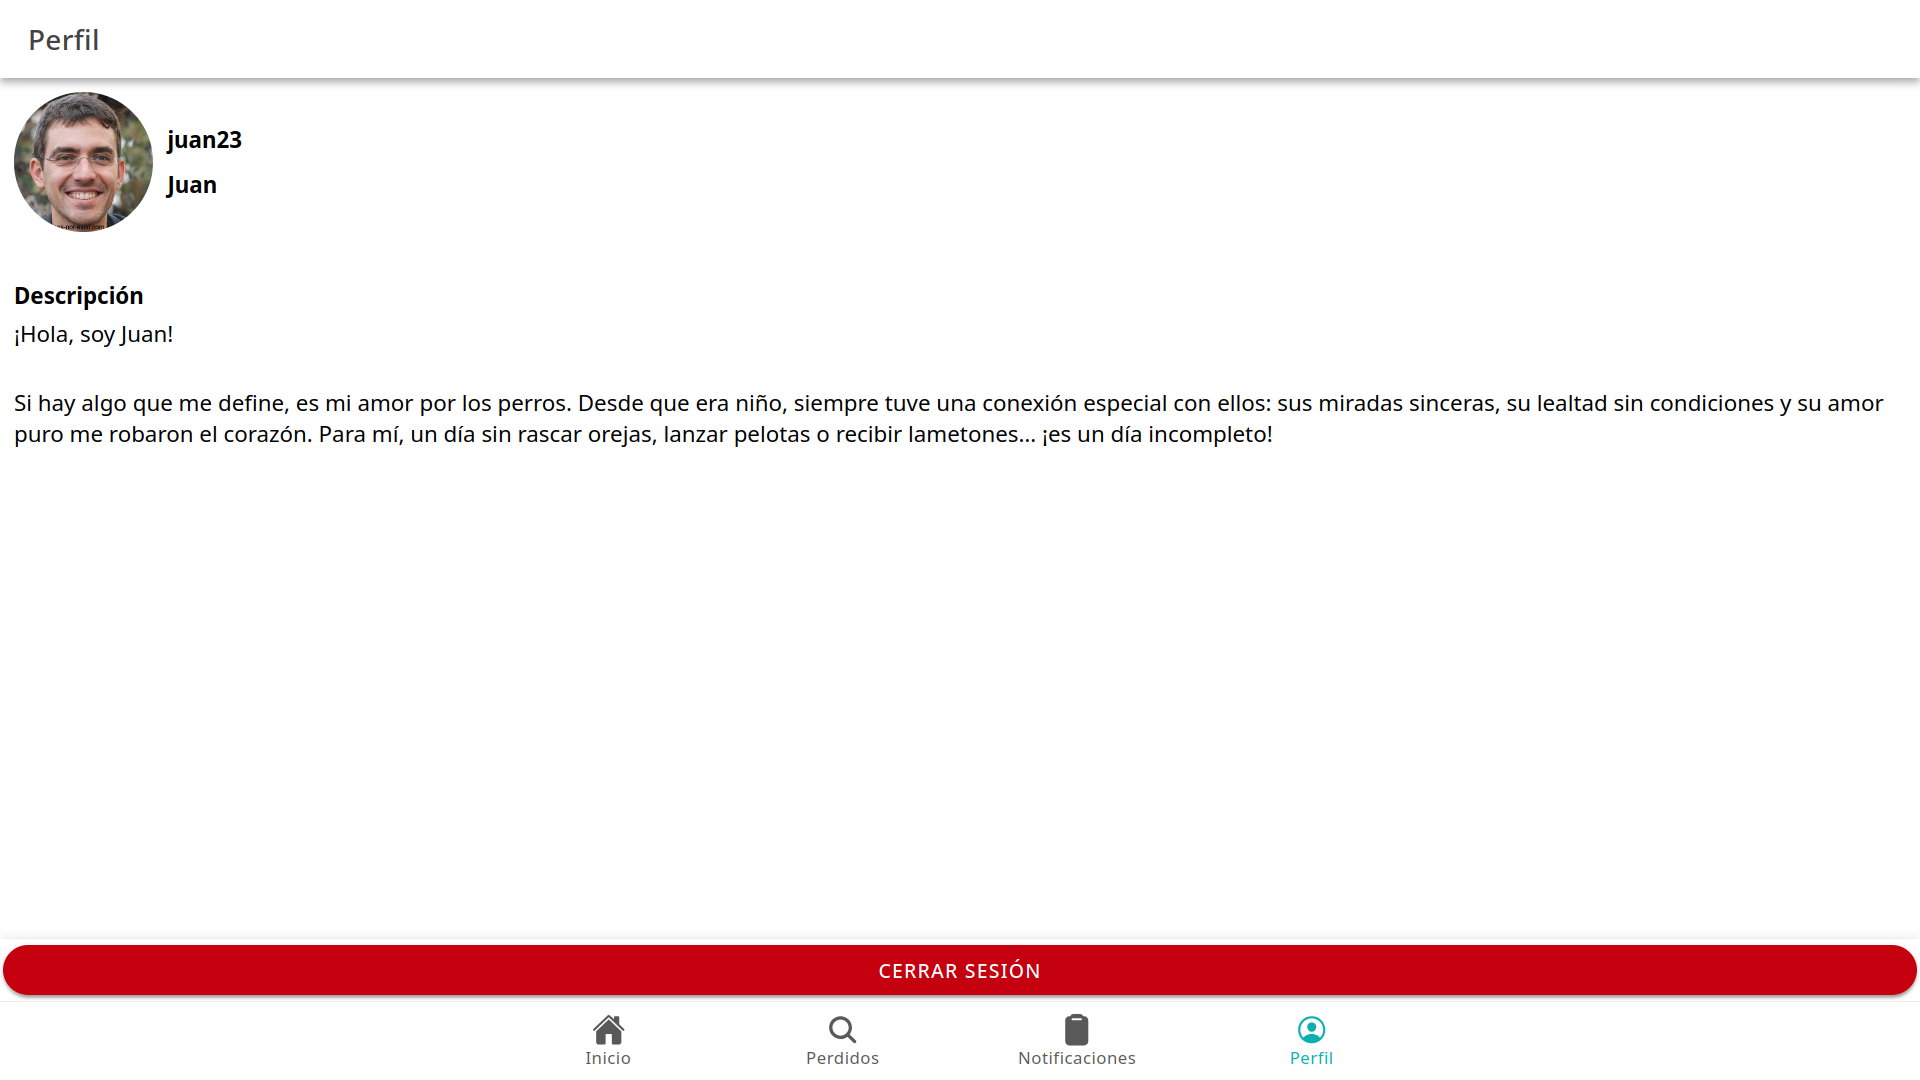
\includegraphics[width=1\linewidth]{sprint 3//hu11-12/implementacionWeb.png}
	\caption{Diseño de la página para ver el perfil en web}
\end{figure}

\Large{\textbf{HU.13 - Buscar particulares que estén como casa de acogida}}

\textbf{Bocetos} \\
\begin{figure}[H]
	\centering
	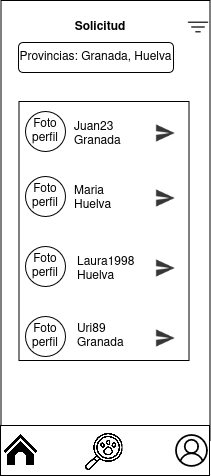
\includegraphics[width=0.31\linewidth]{sprint 3//hu13/boceto.png}
	\caption{Boceto del modal de búsqueda de casas de acogida }
\end{figure}

\textbf{Implementación}

\begin{figure} [H]
	\centering
	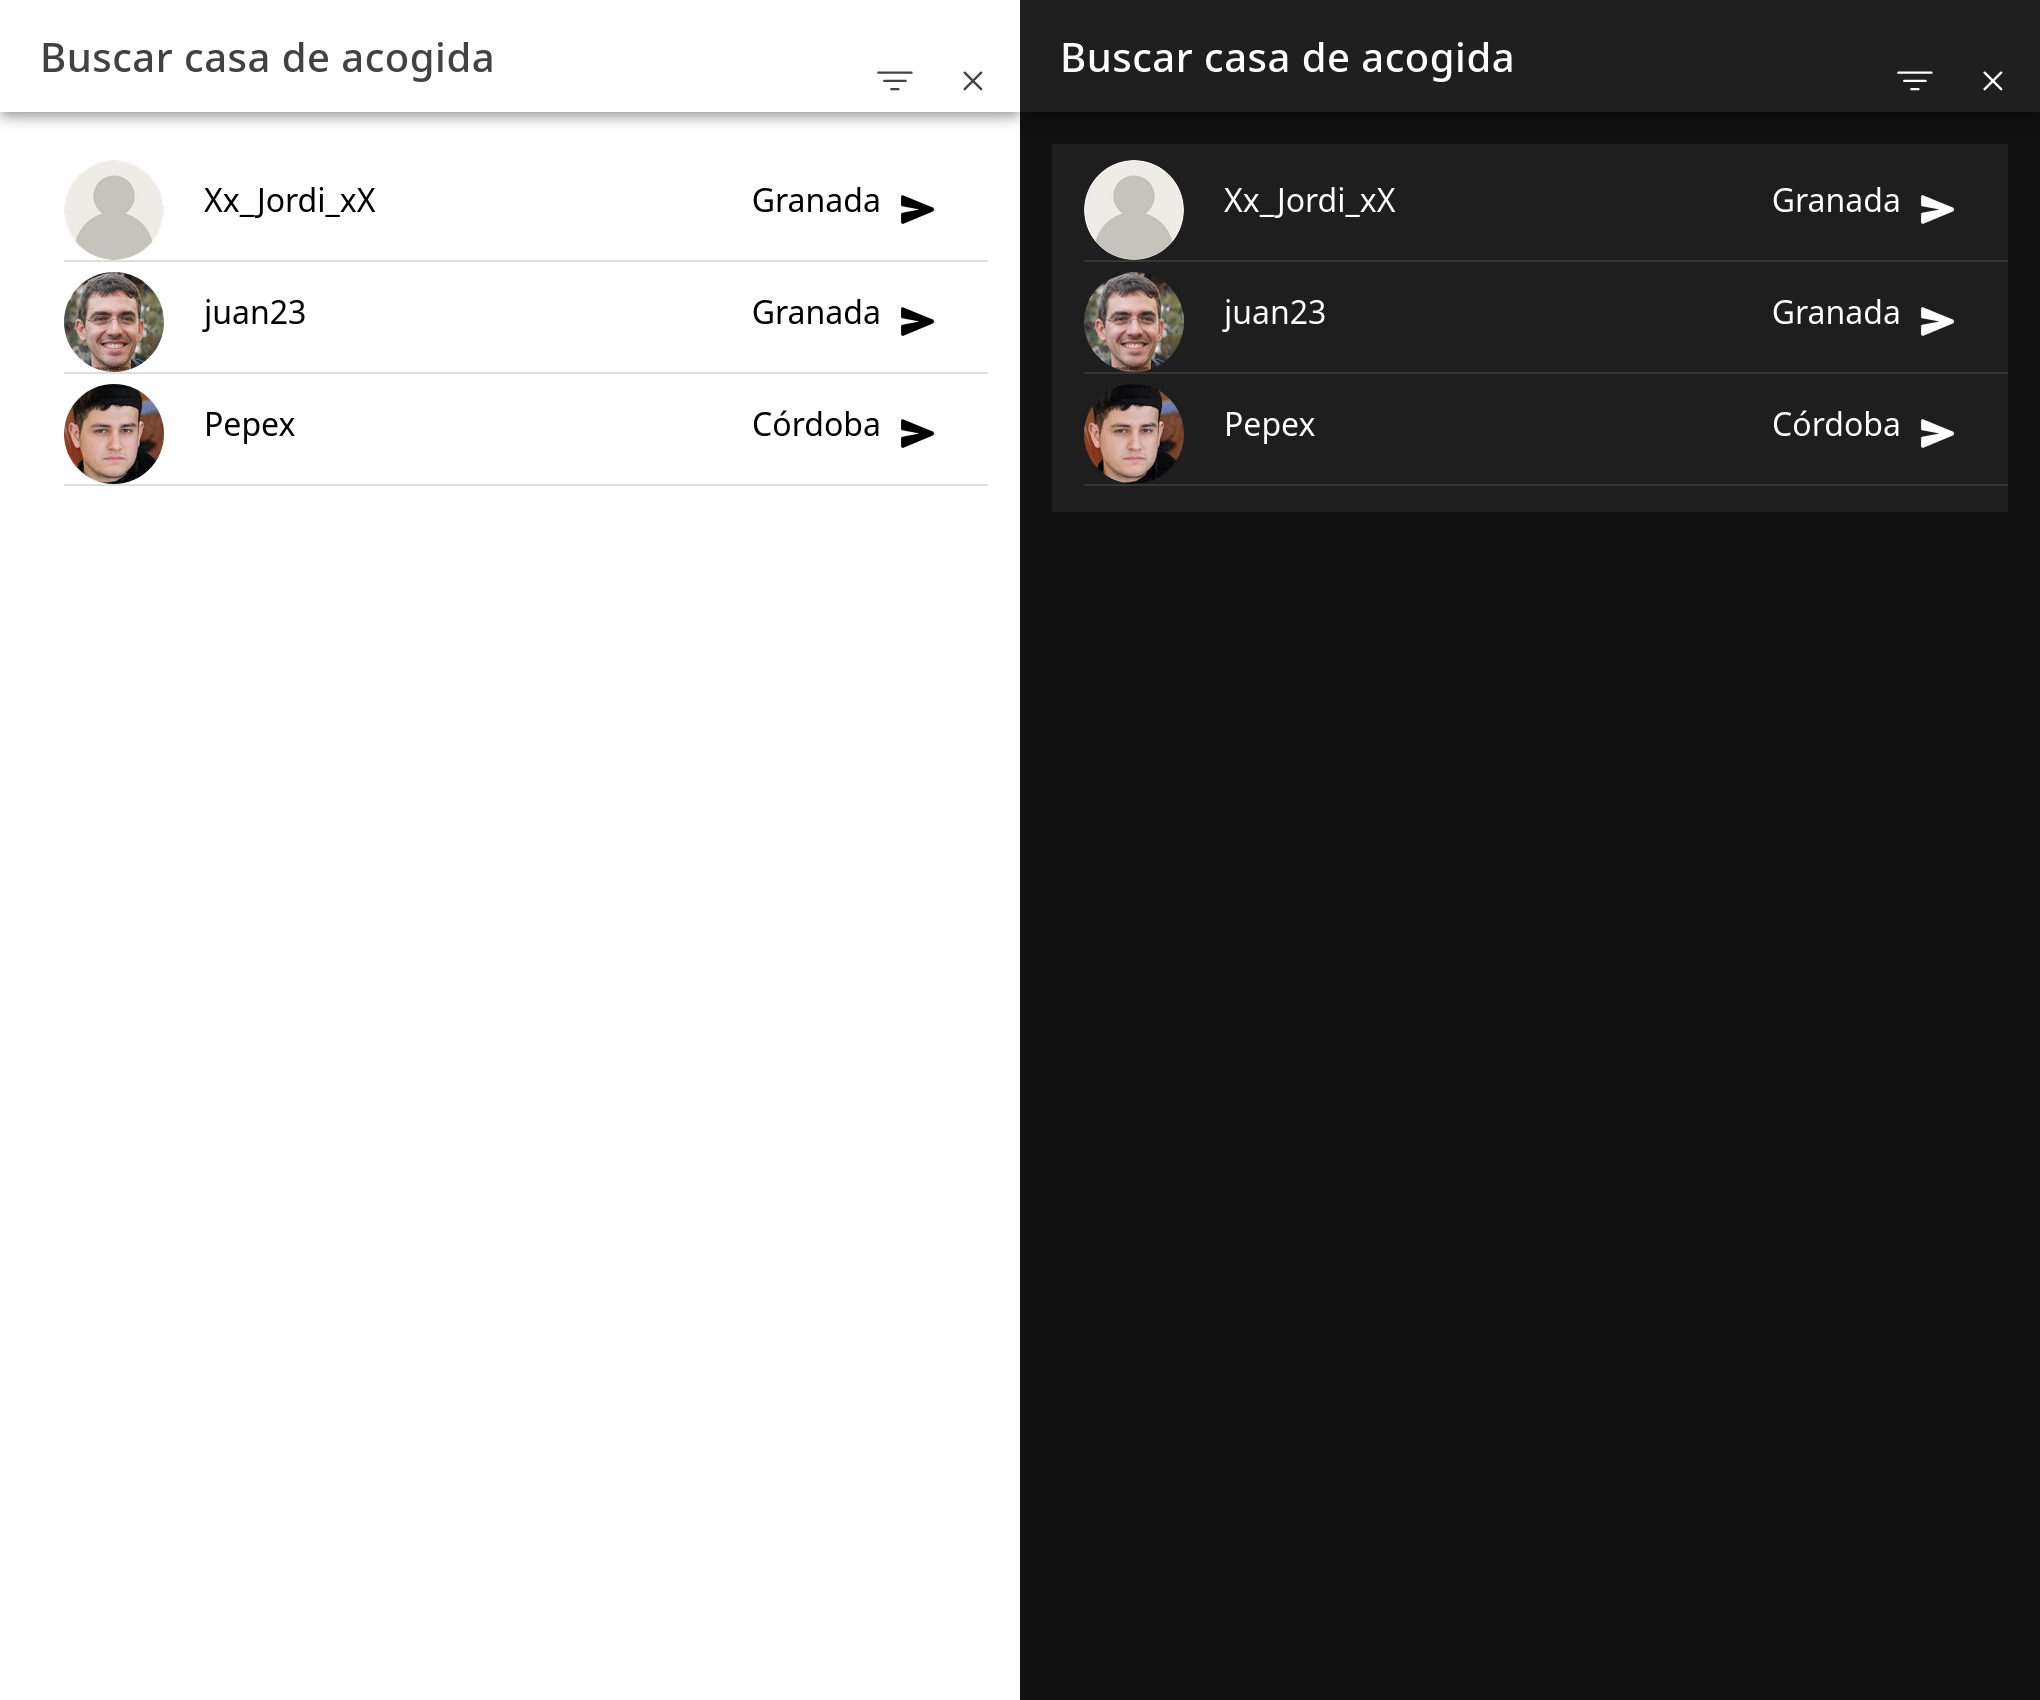
\includegraphics[width=1\linewidth]{sprint 3//hu13/implementacion.png}
	\caption{Diseño del modal de búsqueda de casas de acogida en móviles}
	\label{fig:impBusquedaAcogida}
\end{figure}

\begin{figure}[H]
	\centering
	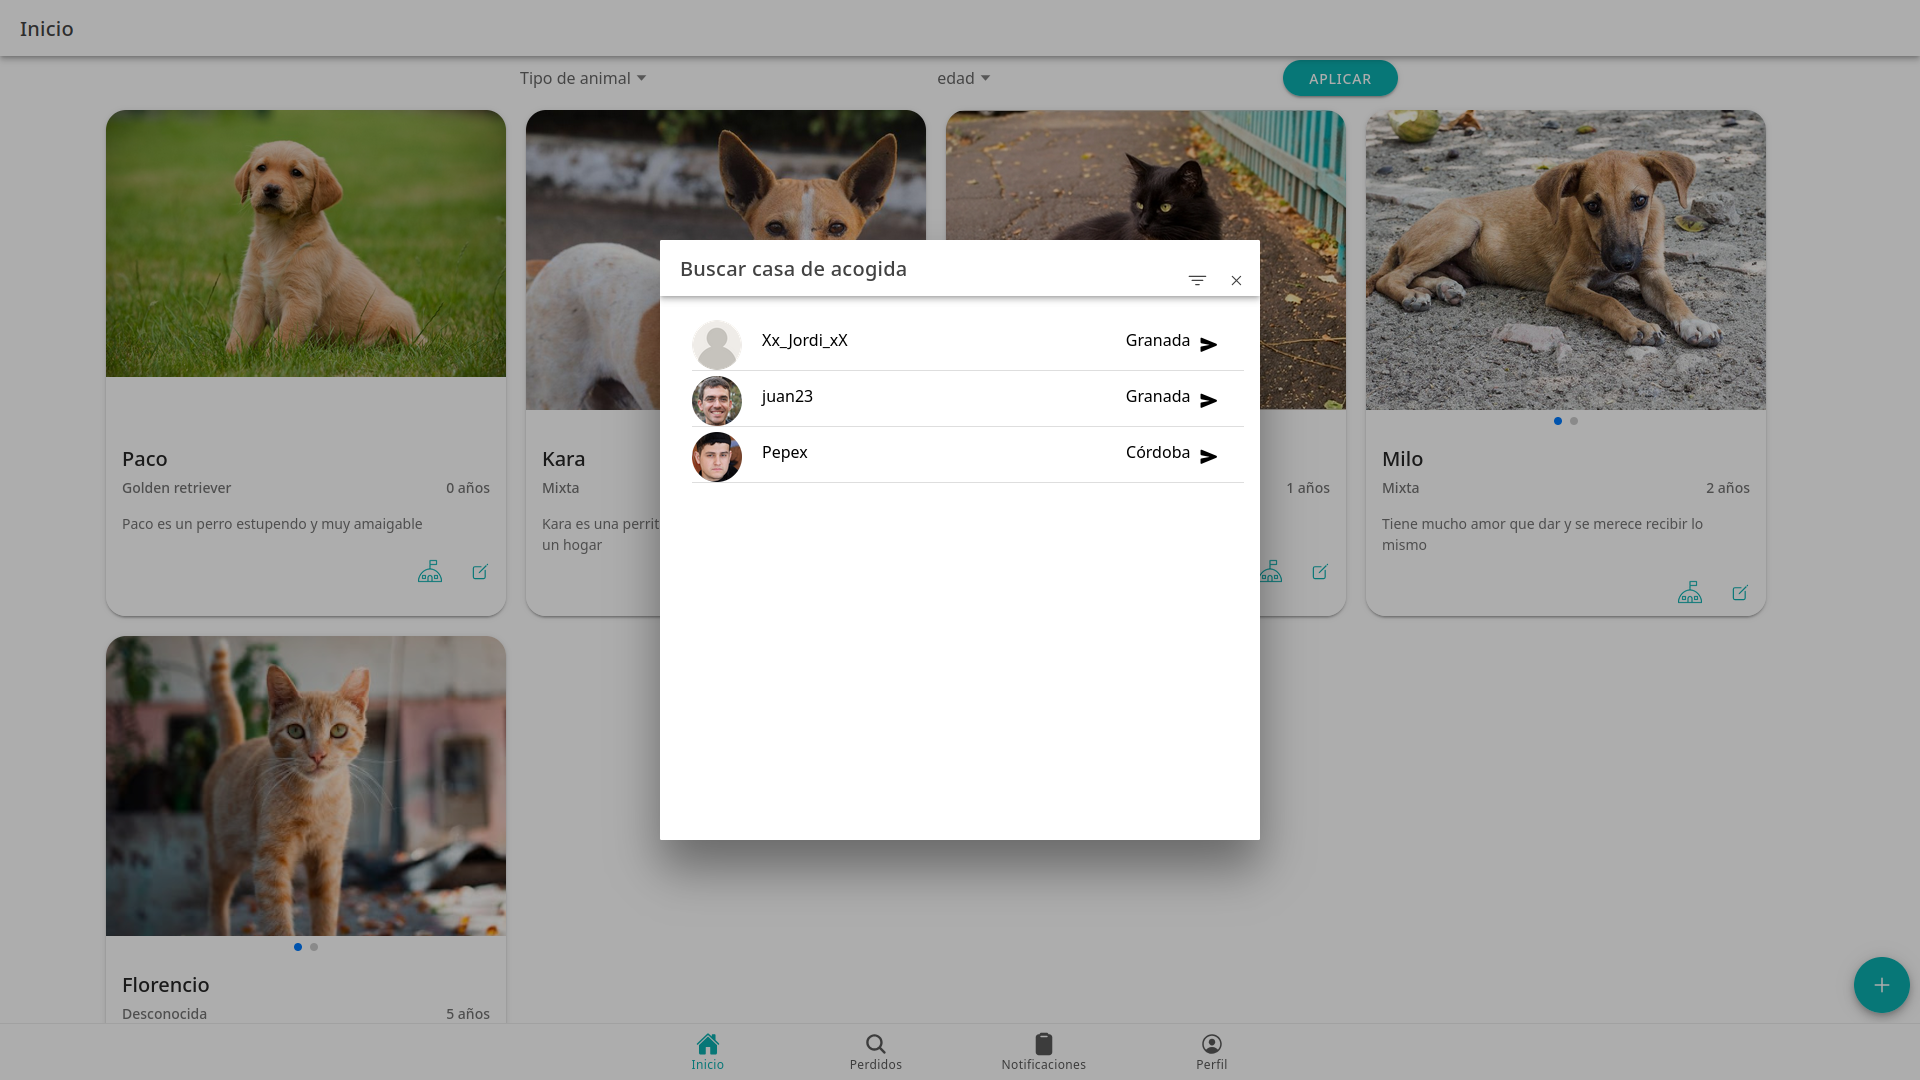
\includegraphics[width=1\linewidth]{sprint 3//hu13/implementacionWeb.png}
	\caption{Diseño del modal de búsqueda de casas de acogida en web}
\end{figure}


Como podemos ver en la figura \ref{fig:impRegAso} el registro de asociaciones utiliza la misma página en el de usuarios estándar en la figura \ref{fig:impregistroparticulares}, simplemente hemos añadido un selector para elegir la opción de registro deseado. Debemos mencionar que en el futuro la creación de asociaciones será revisada por los moderadores y aceptada o denegada por éstos, para ello haremos uso del acta fundacional \cite{actaFundacional}, que es un documento que se necesita a la hora de crear asociaciones. En este documento se encuentra información de relevancia como el NIF, nombre de la asociación, etc.

A consecuencia de esto nos surge la necesidad de encriptar el archivo según la lay de protección de datos, ya que contiene información sensible la cual no debe se accesible desde la base de datos. Para esto hemos usado la librería nativa de node \textit{crypto} \cite{crypto}, la cual nos permite almacenar el archivo encriptado en el servidor de manera segura.

A coalición de lo último hemos tenido que crear la tabla \textit{Files} en la base de datos, la cual contiene el nombre del archivo encriptado y el usuario al que pertenece.


En el proceso de la creación de la página de perfil \ref{fig:impPerfil} se hizo evidente la necesidad de mostrar una pequeña descripción sobre el usuario, por lo que hemos creado el campo \textit{description} en la tabla \textit{Users} de la base de datos.

La búsqueda de casas de acogida nos hizo darnos cuenta de que la página principal de asociaciones debía ser distinta a la de usuarios particulares y básicos. Ahora a las asociaciones en su página principal solo se les muestra sus animales y tienen una serie de botones de acción como el de buscar casa de acogida para ese animal en concreto.



\begin{figure}[H]
	\centering
	\includegraphics[width=0.31\linewidth]{"sprint 3/homeAsociaciones"}
	\caption{Implementación del diseño final de página principal de asociaciones}
	\label{fig:homeasociaciones}
\end{figure}

Al pulsar en el botón de la izquierda se mostrará el modal de búsqueda de asociaciones \ref{fig:impBusquedaAcogida}. Un modal es un cuadro de diálogo que aparece sobre el contenido de la aplicación y que ésta debe cerrar antes de reanudar la interacción.

\textbf{Fin del Sprint}

En esta iteración debido a que se han hecho las tareas en menor tiempo al estimado y por el flujo de la programación se han añadido a mayores la HU-14 y HU-15 que son enviar solicitudes de acogida/adopción y borrarlas respectivamente, incluyendo también el envío de solicitudes de búsqueda de casa de acogida.

Hemos tenido que crear la tabla \textbf{Requests} en la base de datos para almacenar las solicitudes.

También hemos modificado las sesiones, ya que cuando el servidor se caía o apagaba estas desaparecían por completo. Para ello hemos hecho uso de la librería \textit{express-session-mysql} \cite{mysqlSession} la cual aporta persistencia a las sesiones, es decir, se almacenan en la tabla \textit{Sessions} de la base de datos.



La estructura de directorios al final de esta iteración es la siguiente:

\begin{figure}[H]
	\centering
	\includegraphics[width=0.7\linewidth]{"sprint 3/structuraBack"}
	\caption{Estructura de directorios del backend al final del sprint 3}
	\label{fig:structuraback}
\end{figure}

A continuación se muestra el diagrama de clases al final de la tercera iteración con los añadidos que hemos mencionado anteriormente.

\begin{figure}[H]
	\centering
	\includegraphics[width=1\linewidth]{"sprint 3/clases"}
	\caption{Diagrama de clases de la tercera iteración}
	\label{fig:clases3}
\end{figure}


En general hemos ido mejor de lo esperado en la planificación de la iteración, pero es en parte debido a la unión de las páginas de consulta de solicitudes, es decir que las solicitudes de acogida y de adopción finalmente se muestran en la misma página, teniendo todo el sentido ya que tendrían la misma estructura y estética, además de que en la base de datos se almacenan exactamente igual a excepción del tipo de solicitud. 

\subsection{Iteración 4}

En esta última iteración haremos que tanto las asociaciones como los particulares puedan modificar su perfil y la aceptación y rechazo de las solicitudes de adopción y de acogida. También implementaremos la posibilidad de acceder a los perfiles de otros usuarios y de obtener información más detallada de las publicaciones cuando pulsemos en ellas.

Por último en esta iteración también nos encargaremos de solucionar pequeños errores que hemos arrastrado de otras iteraciones, para darle más consistencia a la aplicación. \\ \\

\textbf{Especificación de tareas} \\

\begin{tabular}{|c|p{9.5cm}|p{1cm}|}
	\hline
	\multicolumn{3}{|p{10.5cm}|}{\textbf{HU.17 - Como asociación y usuario particular poder modificar el perfil}} \\
	\hline
	\textbf{Id} & \textbf{Título de la tarea de desarrollo} & \textbf{Est. (días)} \\
	\hline
	17.1 & Realizar bocetos & 0,5 \\ \hline
	17.2 &  Implementar la lógica & 2 \\ \hline
	17.3 &  Implementar la interfaz & 1 \\ \hline
	\multicolumn{3}{|c|}{\textbf{Pruebas de aceptación}} \\ \hline
	1 & \multicolumn{2}{|p{12cm}|}{Que las asociaciones puedan añadir hasta 6 fotos} \\ \hline
	2 & \multicolumn{2}{|p{12cm}|}{Que las imágenes de las asociaciones se puedan modificar, eliminando la imagen modificada de la base de datos} \\ \hline
	3 & \multicolumn{2}{|p{12cm}|}{Que se aplique correctamente la modificación del campo descripción y el resto de campos} \\ \hline
	4 & \multicolumn{2}{|p{12cm}|}{Que los botones de acción realicen correctamente su función} \\ \hline
	
\end{tabular} \\ \\

\begin{tabular}{|c|p{9.5cm}|p{1cm}|}
	\hline
	\multicolumn{3}{|c|}{\textbf{HU.18 - Aceptar solicitudes de adopción}} \\
	\hline
	\textbf{Id} & \textbf{Título de la tarea de desarrollo} & \textbf{Est. (días)} \\
	\hline
	18.1 &  Implementar la lógica & 1 \\ \hline
	18.2 &  Implementar la interfaz & 1 \\ \hline
	\multicolumn{3}{|c|}{\textbf{Pruebas de aceptación}} \\ \hline
	1 & \multicolumn{2}{|p{12cm}|}{Comprobar que el animal adoptado no aparezca en la lista de animales en adopción} \\ \hline
	2 & \multicolumn{2}{|p{12cm}|}{Comprobar que la asociación con el usuario adoptante se realiza correctamente} \\ \hline
	3 & \multicolumn{2}{|p{12cm}|}{Comprobar que se le notifica al usuario que se ha aceptado la adopción} \\ \hline

	
\end{tabular} \\ \\

\begin{tabular}{|c|p{9.5cm}|p{1cm}|}
	\hline
	\multicolumn{3}{|c|}{\textbf{HU.19 - Rechazar solicitudes de adopción}} \\
	\hline
	\textbf{Id} & \textbf{Título de la tarea de desarrollo} & \textbf{Est. (días)} \\
	\hline
	19.1 &  Implementar la lógica & 1 \\ \hline
	19.2 &  Implementar la interfaz & 1 \\ \hline
	\multicolumn{3}{|c|}{\textbf{Pruebas de aceptación}} \\ \hline
	1 & \multicolumn{2}{|p{12cm}|}{Comprobar que se le notifica al usuario que se ha rechazado la adopción} \\ \hline
	
	
\end{tabular} \\ \\


\begin{tabular}{|c|p{9.5cm}|p{1cm}|}
	\hline
	\multicolumn{3}{|c|}{\textbf{HU.20 - Aceptar solicitudes de acogida}} \\
	\hline
	\textbf{Id} & \textbf{Título de la tarea de desarrollo} & \textbf{Est. (días)} \\
	\hline
	20.1 &  Implementar la lógica & 1 \\ \hline
	20.2 &  Implementar la interfaz & 1 \\ \hline
	\multicolumn{3}{|c|}{\textbf{Pruebas de aceptación}} \\ \hline
	1 & \multicolumn{2}{|p{12cm}|}{Comprobar que la asociación con el usuario que acoge se realiza correctamente} \\ \hline
	2 & \multicolumn{2}{|p{12cm}|}{Comprobar que se le notifica al usuario que se ha aceptado la acogida} \\ \hline
	
	
\end{tabular} \\ \\


\begin{tabular}{|c|p{9.5cm}|p{1cm}|}
	\hline
	\multicolumn{3}{|c|}{\textbf{HU.21 - Rechazar solicitudes de acogida}} \\
	\hline
	\textbf{Id} & \textbf{Título de la tarea de desarrollo} & \textbf{Est. (días)} \\
	\hline
	21.1 &  Implementar la lógica & 1 \\ \hline
	21.2 &  Implementar la interfaz & 1 \\ \hline
	\multicolumn{3}{|c|}{\textbf{Pruebas de aceptación}} \\ \hline
	1 & \multicolumn{2}{|p{12cm}|}{Comprobar que se le notifica al usuario que se ha rechazado la acogida} \\ \hline
	
\end{tabular} \\ \\

\begin{tabular}{|c|p{9.5cm}|p{1cm}|}
	\hline
	\multicolumn{3}{|c|}{\textbf{HU.22 - Acceder al perfil del usuario seleccionado}} \\
	\hline
	\textbf{Id} & \textbf{Título de la tarea de desarrollo} & \textbf{Est. (días)} \\
	\hline
	22.1 &  Implementar la lógica & 2 \\ \hline
	22.2 &  Implementar la interfaz & 1 \\ \hline
	\multicolumn{3}{|c|}{\textbf{Pruebas de aceptación}} \\ \hline
	1 & \multicolumn{2}{|p{12cm}|}{Cuando se pulse en un nombre de usuario, te lleve al perfil pertinente} \\ \hline
	2 & \multicolumn{2}{|p{12cm}|}{Si es tu propio perfil te permita editarlo} \\ \hline
	3 & \multicolumn{2}{|p{12cm}|}{En el perfil de las asociaciones aparezcan sus animales en adopción} \\ \hline
	4 & \multicolumn{2}{|p{12cm}|}{Comprobar que no se pueda editar ningún perfil ajeno} \\ \hline
	
\end{tabular} \\ \\

\begin{tabular}{|c|p{9.5cm}|p{1cm}|}
	\hline
	\multicolumn{3}{|c|}{\textbf{HU.23 - Acceder a la publicación ampliada}} \\
	\hline
	\textbf{Id} & \textbf{Título de la tarea de desarrollo} & \textbf{Est. (días)} \\
	\hline
	23.1 &  Implementar la lógica & 2 \\ \hline
	23.2 &  Implementar la interfaz & 1,5 \\ \hline
	\multicolumn{3}{|c|}{\textbf{Pruebas de aceptación}} \\ \hline
	1 & \multicolumn{2}{|p{12cm}|}{Cuando se pulse en una publicación, accedas a la misma con la información ampliada} \\ \hline
	2 & \multicolumn{2}{|p{12cm}|}{Comprobar que los botones de acción funcionan correctamente} \\ \hline
	3 & \multicolumn{2}{|p{12cm}|}{Comprobar que un usuario no registrado no pueda solitar adopción ni acogida} \\ \hline
	
\end{tabular} \\ \\


\begin{tabular}{|c|p{9.5cm}|p{1cm}|}
	\hline
	\multicolumn{3}{|c|}{\textbf{HU.24 - Resolución de errores}} \\
	\hline
	\textbf{Id} & \textbf{Título de la tarea de desarrollo} & \textbf{Est. (días)} \\
	\hline
	24.1 & Arreglar que solo se pueda subir una imagen a la hora de subir publicaciones  & 1 \\ \hline
	24.2 &  Arreglar problema de scroll & 0,5 \\ \hline
	24.3 &  Mantenerte loggeado cuando te acabas de registrar como usuario particular & 0,5 \\ \hline
\end{tabular} \\ \\


\Large{\textbf{HU.17 - Como asociación y usuario estándar poder modificar el perfil}}

\textbf{Bocetos}

\begin{figure}[H]
	\centering
	\includegraphics[width=0.31\linewidth]{"sprint 4/hu17/editarPerfil"}
	\caption{Boceto de la página de editar perfil}
	\label{fig:editarperfil}
\end{figure}

\textbf{Implementación}


\begin{figure}[H]
	\centering
	\includegraphics[width=1\linewidth]{"sprint 4/hu17/implementacion"}
	\caption{Implementación de la página de editar perfil en móviles}
	\label{fig:implementacionEditarPerfil}
\end{figure}


\begin{figure}[H]
	\centering
	\includegraphics[width=1\linewidth]{"sprint 4/hu17/implementacionWeb"}
	\caption{Implementación de la página de editar perfil en web}
	\label{fig:implementacionEditarPerfilWeb}
\end{figure}


\Large{\textbf{HU.18, HU.19, HU.20, HU.21 - Aceptar/Rechazar solicitudes de adopción/acogida }} \\

En estas historias no se requiere realización de bocetos ni de diseño ya que para aceptar y/o rechazar solicitudes usaremos la página de notificaciones vista anteriormente en la figura \ref{fig:notificaciones}. 

Cabe destacar que hemos cambiado el nombre de la página de solicitudes a notificaciones, ya que en esta misma también se le avisará a las asociaciones y los usuarios particulares del estado final de sus solicitudes.

\begin{figure}[H]
	\centering
	\includegraphics[width=0.5\linewidth]{"sprint 4/hu17/notificacionesNueva"}
	\caption{Página de notificaciones con el cambio de nombre}
	\label{fig:notificacionesnueva}
\end{figure}


\Large{\textbf{HU.23 - Acceder a la publicación ampliada}}

\textbf{Bocetos}

\begin{figure}[H]
	\centering
	\includegraphics[width=0.31\linewidth]{"sprint 4/hu23/publicacionAmpliada"}
	\caption{boceto de la página de publicación ampliada}
	\label{fig:publicacionampliada}
\end{figure}

\textbf{Implementación}
\begin{figure}[H]
	\centering
	\includegraphics[width=1\linewidth]{"sprint 4/hu23/impPublicaciónAmpliada"}
	\caption{Implementación de la página de publicación ampliada en móviles}
	\label{fig:imppublicacionampliada}
\end{figure}

\begin{figure}[H]
	\centering
	\includegraphics[width=1\linewidth]{"sprint 4/hu23/publicacionAmpliadaWeb"}
	\caption{Implementación de la página de publicación ampliada en web}
	\label{fig:publicacionampliadaweb}
\end{figure}

En esta última iteración como hemos visto, se han realizado implementaciones de las notificaciones y de vista de perfiles principalmente. 

Además este ha sido el sprint en el que hemos hecho algunas correcciones finales más que ampliando funcionalidades primando la estabilidad de la aplicación frente a la cantidad de contenido añadido.

Por ejemplo se ha solucionado la obtención de las provincias de un país en la página principal del los usuarios estándar, para ello hemos hecho uso de una api \cite{apiIp} la cual nos devuelve información del país en función de la dirección ip que tengamos asignada. Esto nos permite saber la localización aproximada del dispositivo sin tener que solicitar permisos de ubicación.

Para que esto funcionase se ha modificado la tabla de países en la base de datos añadiéndole el campo \textit{code} para que la búsqueda sea posible, además también hemos puesto los nombres de dichos países en 3 de los principales idiomas: español, inglés y francés cada uno con sendos campos en la base de datos y solo obteniendo en las consultas aquel que sea necesario, en caso de no tener el dispositivo en ninguno de esos idiomas se obtienen los nombres en inglés.

También hemos creado en la base de datos la tabla \textit{AsoSpecies} la cual refleja la relación de muchos a muchos que hay entre las asociaciones y las distintas especies. Gracias a esto ahora una asociación puede tener en adopción distintos tipos de animales y además se les ha añadido la posibilidad de avisar a los usuarios que también permiten acogidas de animales en la propia  asociación. Todo esto se puede modificar con los selectores que aparecen al querer editar el perfil como se muestra en la figura \ref{fig:implementacionEditarPerfil}.

Por último, con respecto al perfil ahora cuando accedamos a alguno se nos indica que características tiene éste mediante etiquetas. Con esto permitimos que con un vistazo rápido se pueda obtener información básica sobre los perfiles.

\begin{figure}[H]
	\centering
	\includegraphics[width=0.5\linewidth]{"sprint 4/etiquetasPerfil"}
	\caption{Implementación de las etiquetas al  visualizar un perfil}
	\label{fig:etiquetasperfil}
\end{figure}

La estructura final de los directorios quedaría de esta manera:
\begin{figure}[H]
	\centering
	\includegraphics[width=0.7\linewidth]{"sprint 4/directorios"}
	\caption{Estructura de directorios del backend al final del sprint 4}
	\label{fig:directorios4}
\end{figure}

A continuación se muestra el diagrama de clases al final de la cuarta iteración con los añadidos que hemos mencionado anteriormente.


\begin{figure}[H]
	\centering
	\includegraphics[width=1\linewidth]{"sprint 4/clases"}
	\caption{Diagrama de clases de la cuarta iteración}
	\label{fig:clasesCuarta}
\end{figure}

A nivel de temporalización hemos ido según lo esperado terminando la iteración dentro de lo estimado y sin ningún problema reseñable.















